% Chapter 12

\chapter{Final charged hadrons multiplicities} % Chapter title

\label{ch:mult} % For referencing the chapter elsewhere, use \autoref{ch:name}

%----------------------------------------------------------------------------------------

This chapter is divided in two parts : one is focused on the discussion on the systematic uncertainties, the other presents the final multiplicities of unidentified charged hadrons, charged pions, charged kaons and protons/antiprotons extracted from SIDIS of $160$ GeV muons off a pure proton target ($lH_2$). These results are obtained from the raw multiplicities of Chapter. \ref{ch:raw} and the correction factors of Chapter. \ref{ch:CF}.

%----------------------------------------------------------------------------------------

\section{Summary of systematic studies}

The various systematic studies that were performed are summarized hereafter.

%----------------------------------------------------------------------------------------

\subsection{Systematic uncertainty associated to the RICH unfolding}

The first stage of pion identification is based on the likelihood ratios : $LH(\pi)/LH(2^{nd})$ and $LH(\pi)/LH(bg)$. These cuts are optimized to minimize the
pions misidentified as kaons. The systematic error associated to the selection of these cuts is performed varying the cuts around optimized values. Two sets of
cuts \textit{loose} and \textit{severe} were used (see Table~\ref{tab:loose.severe})

\begin{table}[!h]
	\centering
	\begin{tabular}{ccccccc}
		\hline
		 & \multicolumn{3}{c}{Loose} & \multicolumn{3}{c}{Severe} \\
		\hline
		 & $\pi$ & $K$ & $p(\bar{p})$ & $\pi$ & $K$ & $p(\bar{p})$ \\
		\hline
		$\frac{LH(\pi)}{LH(2^{nd})}$ & $> 1.00$ & $-$ & $-$ & $>1.06$ & $-$ & $-$ \\
		$\frac{LH(\pi)}{LH(bg)}$ & $> 2.00$ & $-$ & $<2.3$ $(2.2)$ & $>2.04$ & $-$ & $<2.0$ $(1.9)$ \\
		$\frac{LH(K)}{LH(2^{nd})}$ & $-$ & $>1.06$ & $-$ & $>-$ & $>1.10$ & $-$ \\
		$\frac{LH(K)}{LH(bg)}$ & $-$ & $>2.00$ & $<3.0$ $(2.9)$ & $-$ & $>2.16$ & $<2.7$ $(2.6)$ \\
		\hline
	\end{tabular}
  \caption{Set of loose and severe cuts to evaluate the RICH systematic errors.}
  \label{tab:loose.severe}
\end{table}

To evaluate the systematic error associated to the selection of the particle likelihood cuts, the particle identification is performed using the \textit{loose}
and \textit{severe} sets of likelihood cuts and the corresponding RICH probability matrices and final multiplicities are extracted ($M^{h^{\pm},loose}_{raw}$
and $M^{h^{\pm},severe}_{raw}$ respectively). The largest difference between $M^{h^{\pm},loose}_{raw}$ and $M^{h^{\pm},severe}_{raw}$ with the nominal
multiplicity $M^{h^{\pm}}_{raw}$ is taken as an estimate of the systematic error :
%
\begin{equation}
  \sigma^{RICH_{LH}}_{sys} = MAX(|M^{h^{\pm},loose}_{raw}-M^{h^{\pm}}_{raw}|,|M^{h^{\pm},severe}_{raw}-M^{h^{\pm}}_{raw}|).
\end{equation}
%
The difference between the altered RICH probability matrices and the optimal one are plotted in Figs.~\ref{pic:Sysplus} and \ref{pic:Sysminus}. For pions and protons, the largest differences
($<5$\%) are observed in the high momentum $p_h$ region. For kaons the difference reaches $4$\% at low $p_h$ ; small differences ($<1$\%) are observed at the
highest $p_h$ value.

A second source of systematic error is that associated with the calculation of the RICH probability matrices. This is estimated by generating two sets of altered
RICH probability matrices. As represented in Eq.~\ref{eq:StatMat} the matrices are constructe using the statistical error associated to the original probability matrix elements.

\begin{figure}[!p]
	\centering
	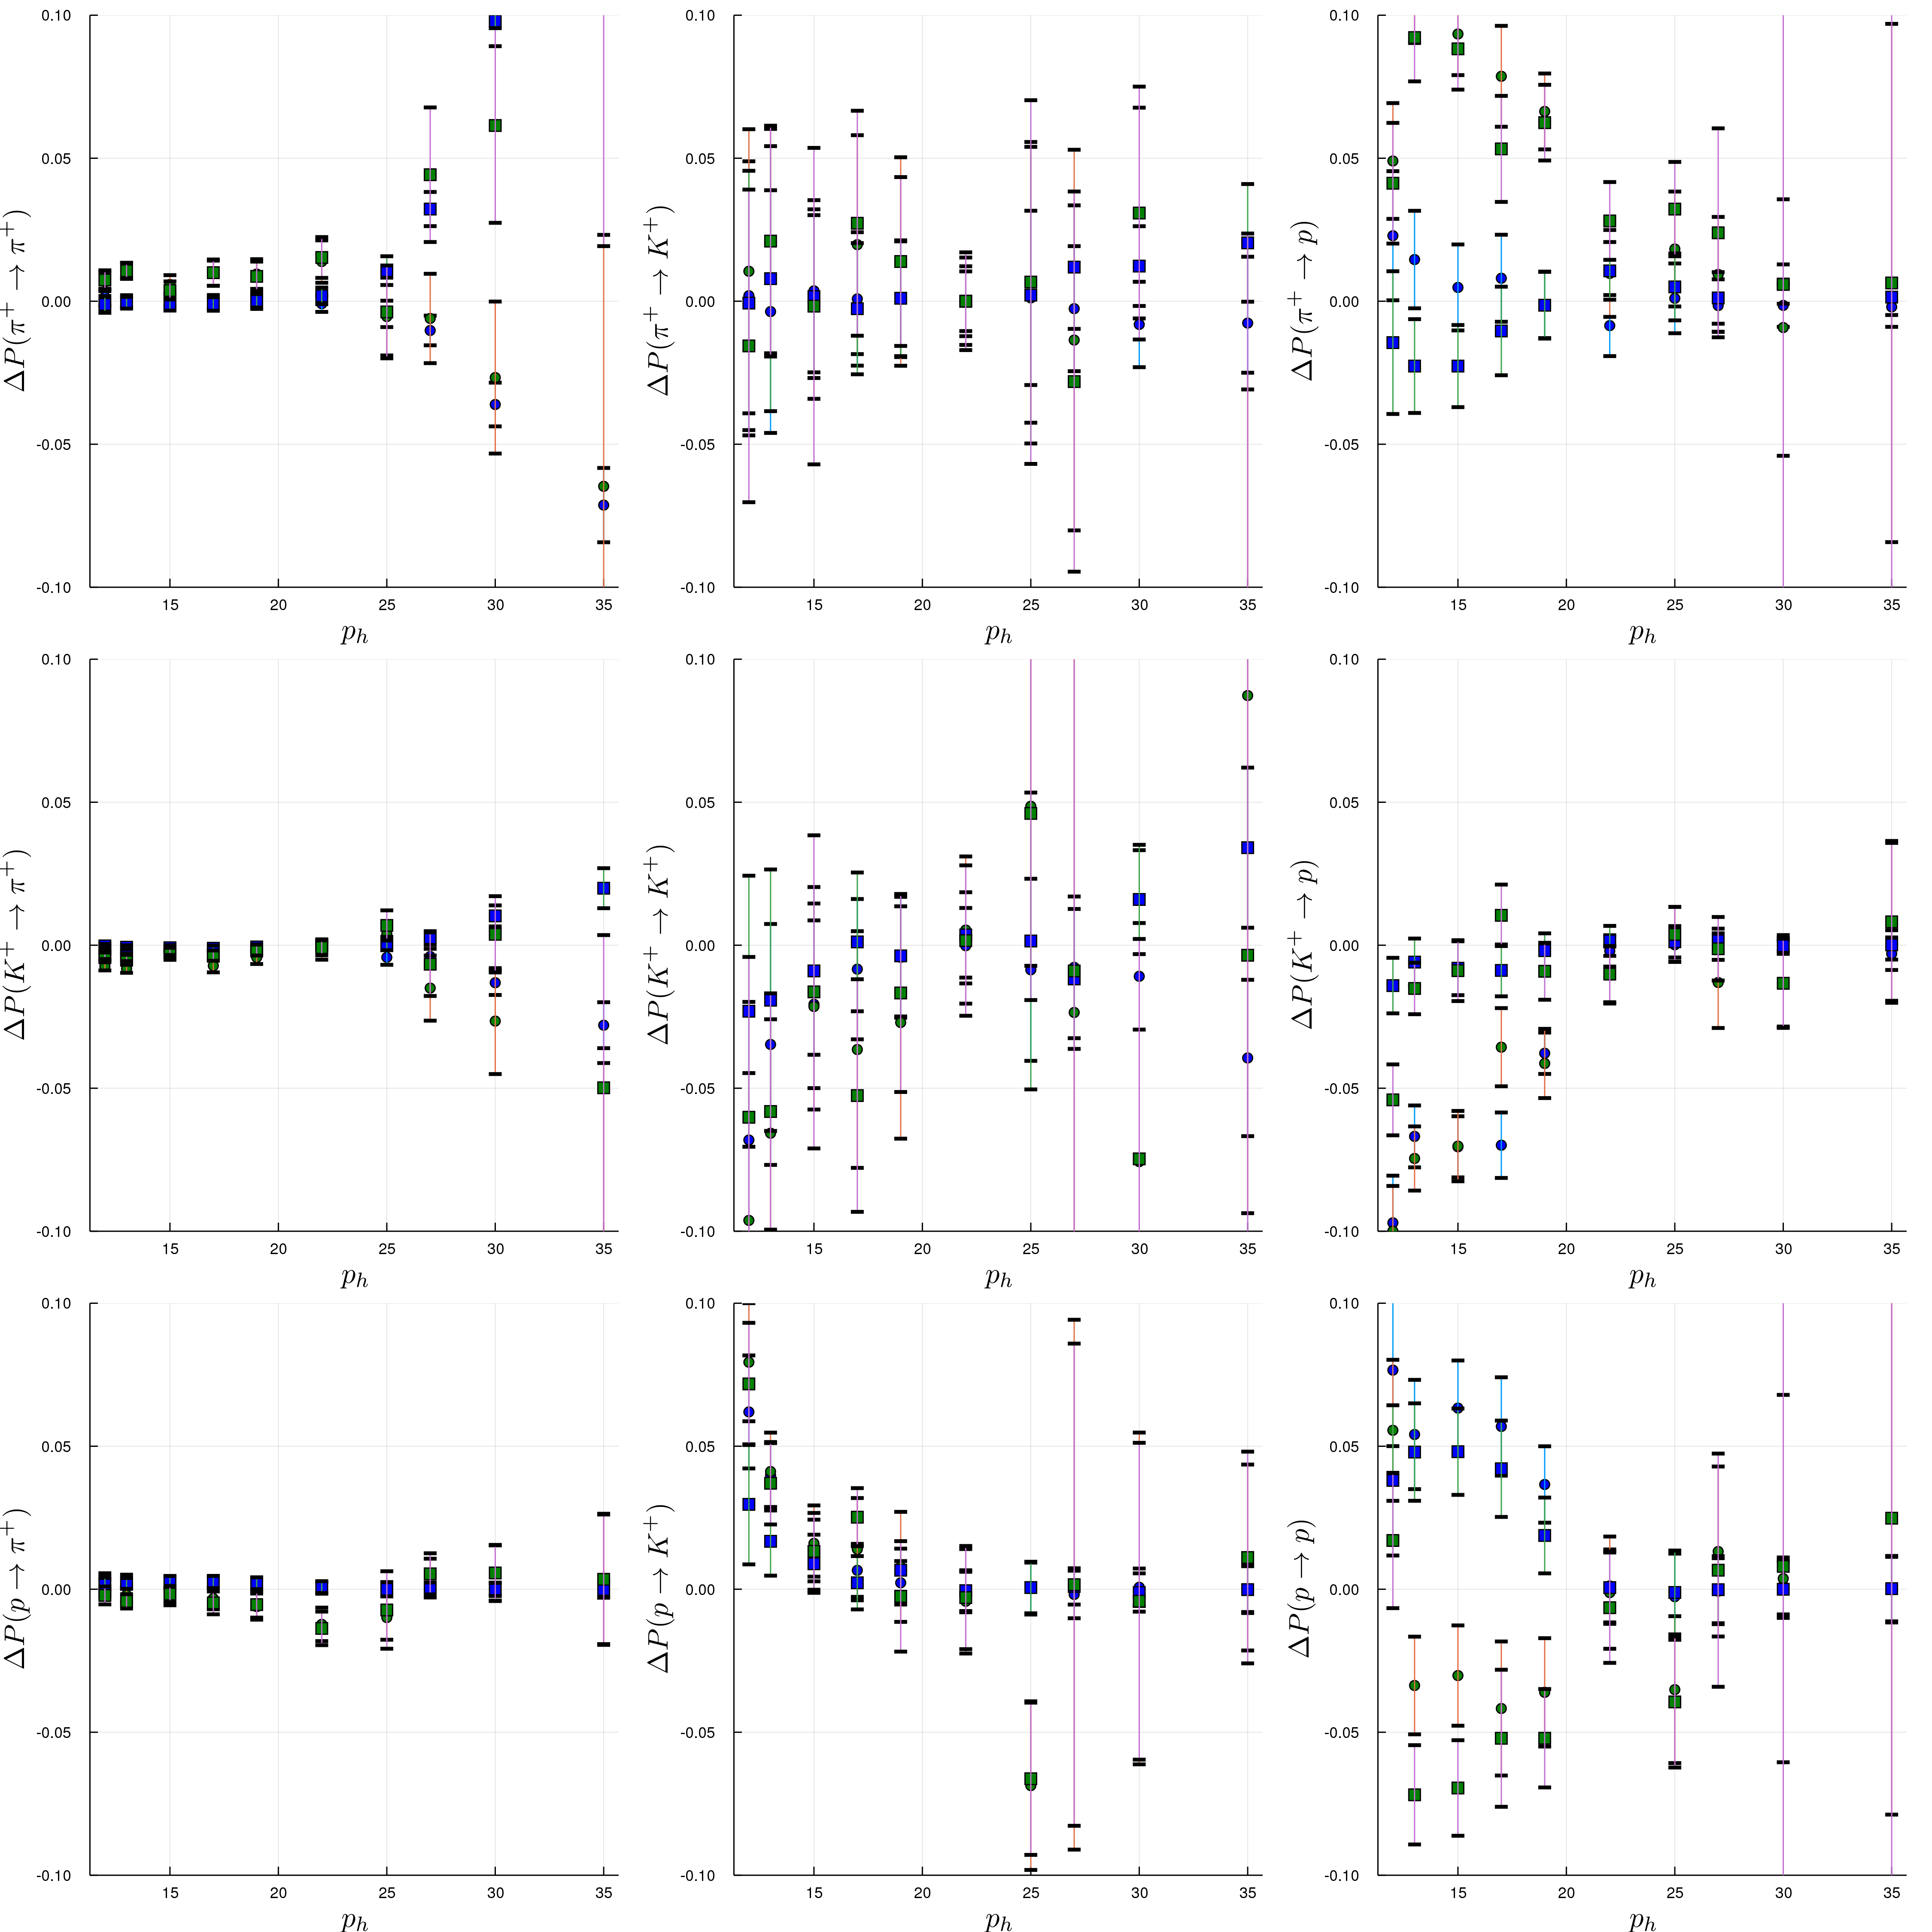
\includegraphics[scale=0.1]{./gfx/SysPlus.png}
	\caption{Difference between the identification and misidentification probabilities of loose and severe cuts with the optimal cuts for positive hadrons.}
	\label{pic:Sysplus}
\end{figure}

\begin{figure}[!p]
	\centering
	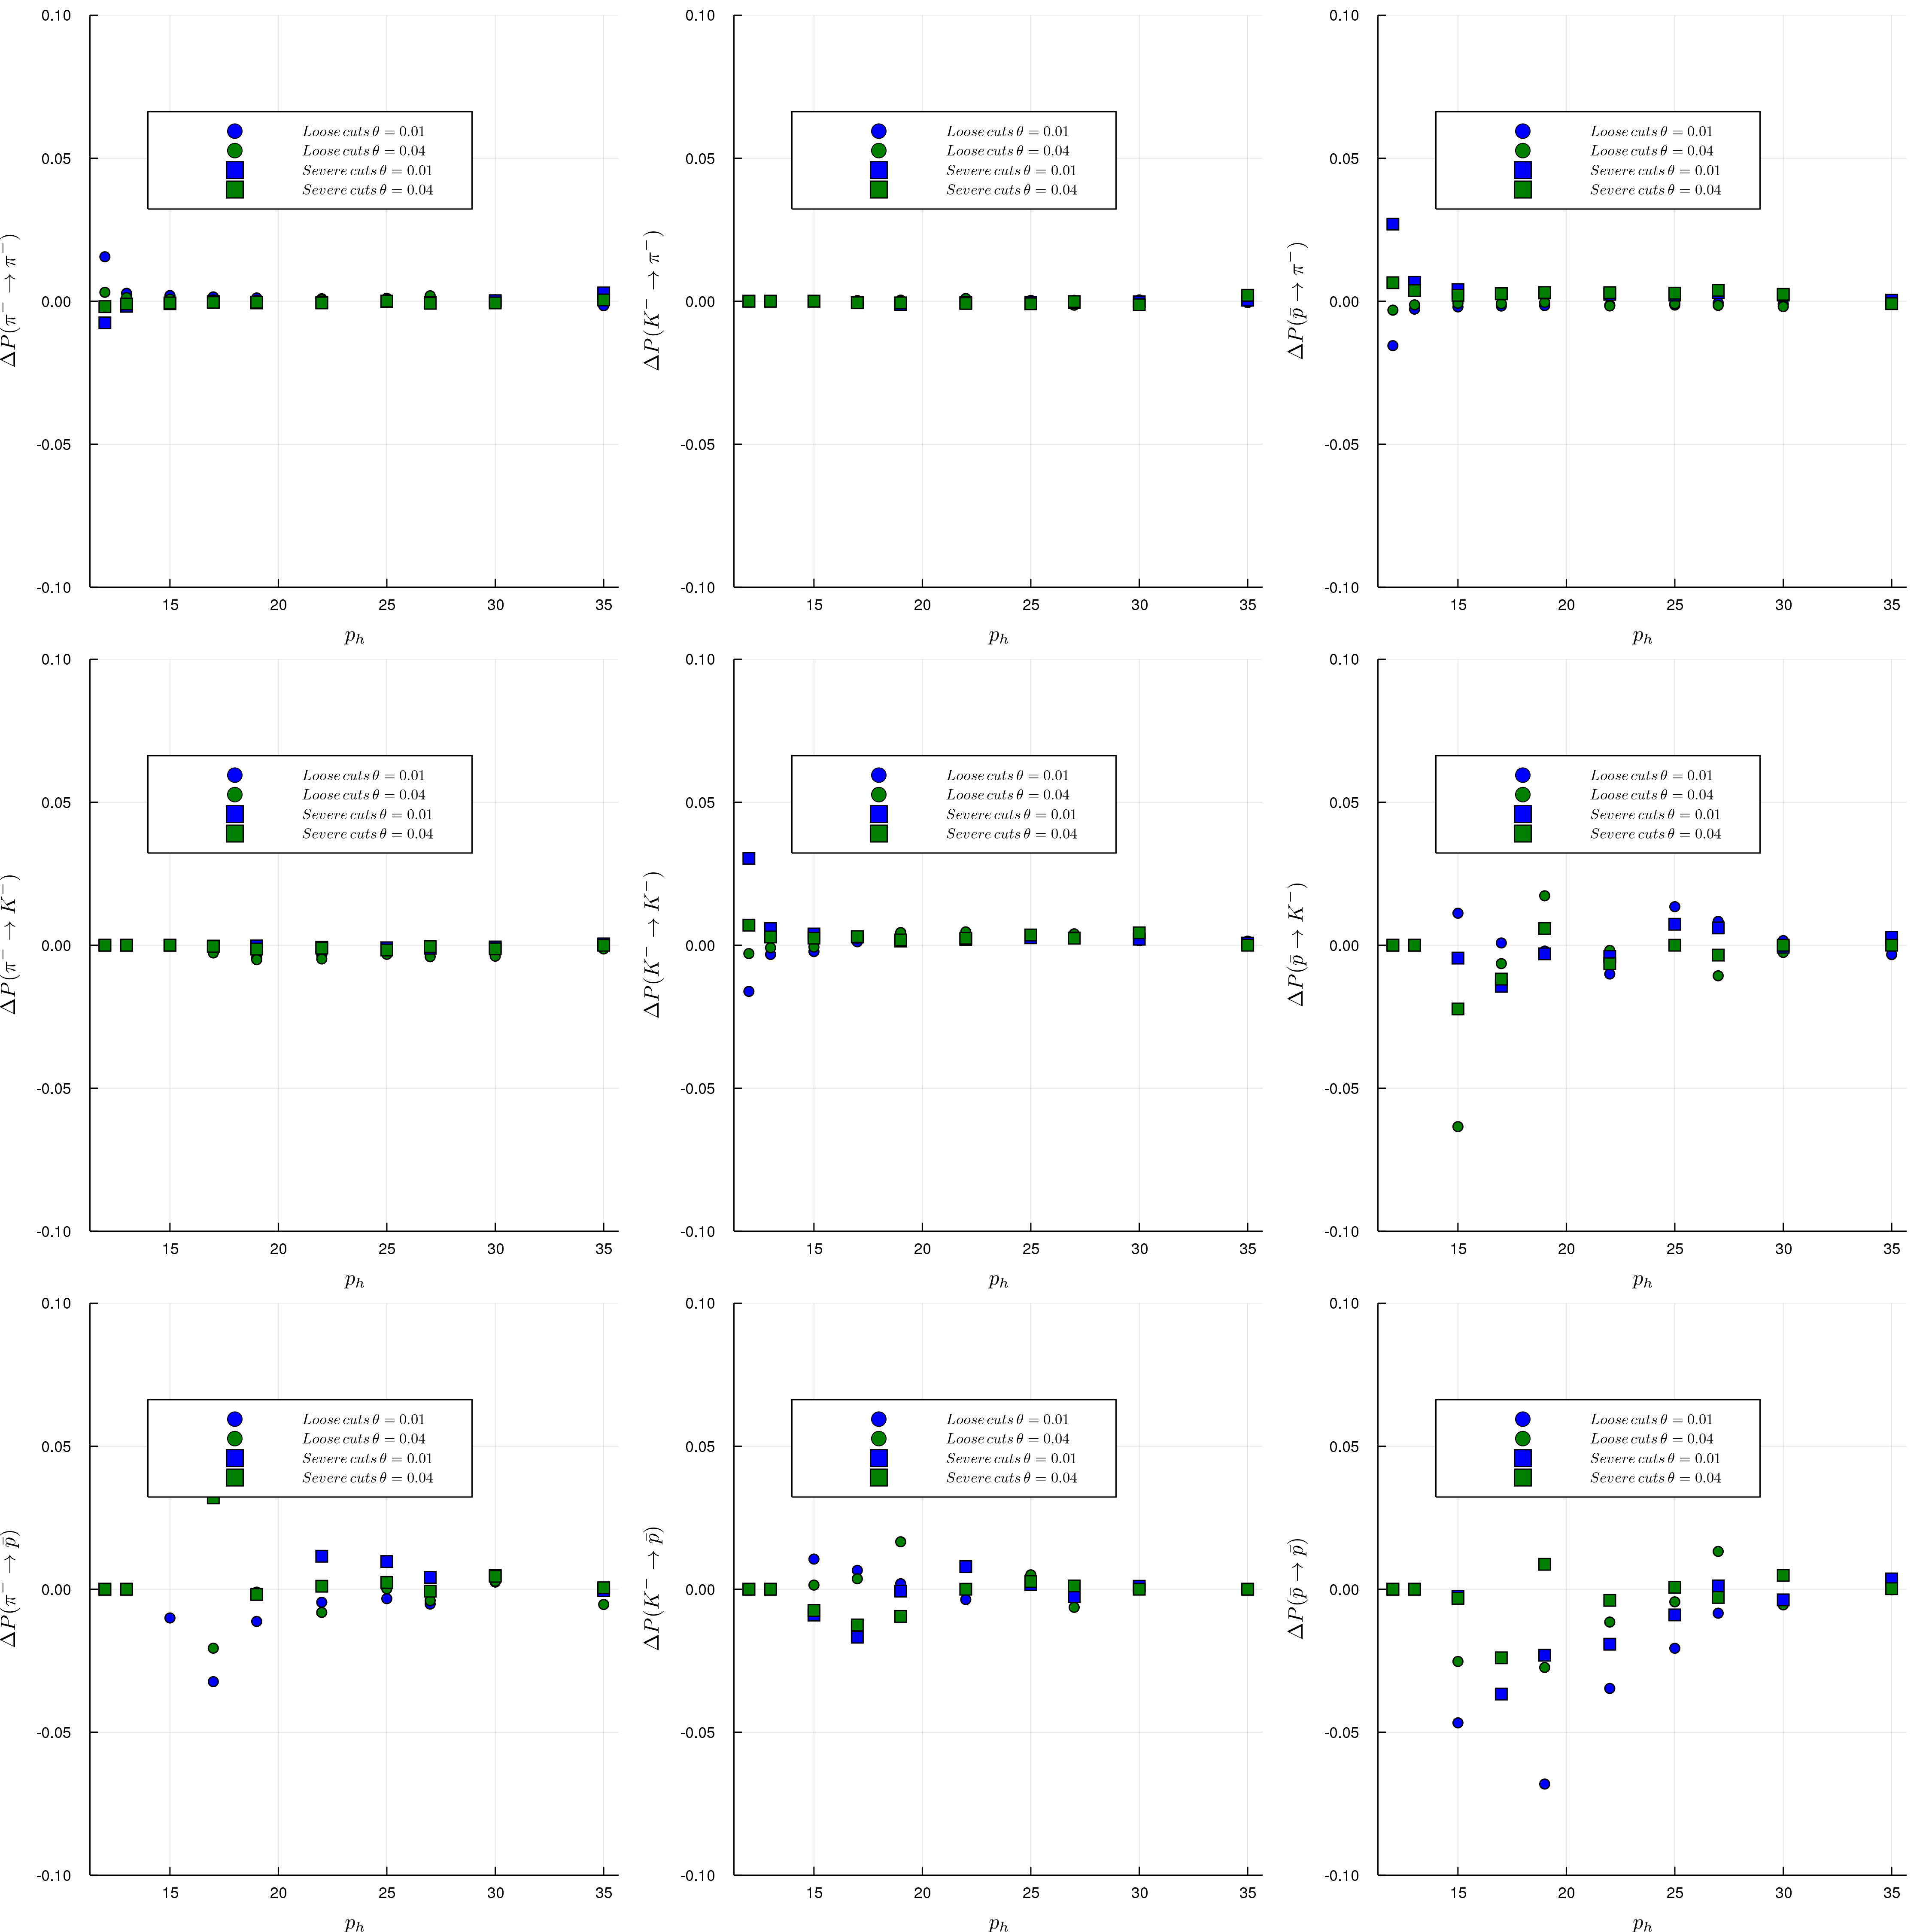
\includegraphics[scale=0.1]{./gfx/SysMinus.png}
	\caption{Difference between the identification and misidentification probabilities of loose and severe cuts with the optimal cuts for negative hadrons.}
	\label{pic:Sysminus}
\end{figure}
%
\begin{equation}
  M^{\pm}_{RICH}
  =
  \begin{bmatrix}
  P(\pi \rightarrow \pi)\pm\sigma_{P(\pi \rightarrow \pi)} & P(K \rightarrow \pi)\mp\sigma_{P(K \rightarrow \pi)} & P(p \rightarrow \pi)\mp\sigma_{P(p \rightarrow \pi)}\\
  P(\pi \rightarrow K)\mp\sigma_{P(\pi \rightarrow K)} & P(K \rightarrow K)\pm\sigma_{P(K \rightarrow K)} & P(p \rightarrow K)\mp\sigma_{P(p \rightarrow K)} \\
  P(\pi \rightarrow p)\mp\sigma_{P(\pi \rightarrow p)} & P(K \rightarrow p)\mp\sigma_{P(K \rightarrow p)} & P(p \rightarrow p)\pm\sigma_{P(p \rightarrow p)}
  \end{bmatrix}
	\label{eq:StatMat}
\end{equation}
%
The raw multiplicities $M^{h^{\pm},+}_{raw}$ and $M^{h^{\pm},-}_{raw}$ are then recalculated using the altered probability matrices. The largest difference between
$M^{h^{\pm},+}_{raw}$ and $M^{h^{\pm},-}_{raw}$ with $M^{h^{\pm}}_{raw}$ is taken as the sytematic error :
%
\begin{equation}
  \sigma^{RICH_{stat}}_{sys} = MAX(|M^{h^{\pm},+}_{raw}-M^{h^{\pm}}_{raw}|,|M^{h^{\pm},-}_{raw}-M^{h^{\pm}}_{raw}|).
\end{equation}
%
The final systematic uncertainty associated to the particle identification and unfolding correction ($\sigma^{RICH}_{sys}$) is the largest value of $\sigma^{RICH_{stat}}_{sys}$ and $\sigma^{RICH_{LH}}_{sys}$. The error goes from $<$ $0.2$\% at low $y$ for all $x$ and $z$ bins to $\sim$ $20$\% for high $y$ and high $z$, where multiplicities are low.

%------------------------------------------------

\subsection{Systematic uncertainty associated to the stability of data over time}

The data samples used in the analysis were recorded over a period of $5$ weeks. As a quality check, the raw charged hadron multiplicities from period P$07$ and from all periods (averaged using the flux as weight) were compared. The results were found to be be compatible within statistical fluctuations for all unidentified hadrons, pions, kaons and protons (Fig.~\ref{pic:hMultTime} for unidentified hadrons, other species in Appendix~\ref{app:Sys}). Consequently, no systematic error will be assigned for the data compatibility.

\begin{sidewaysfigure}[p]
  \centering
	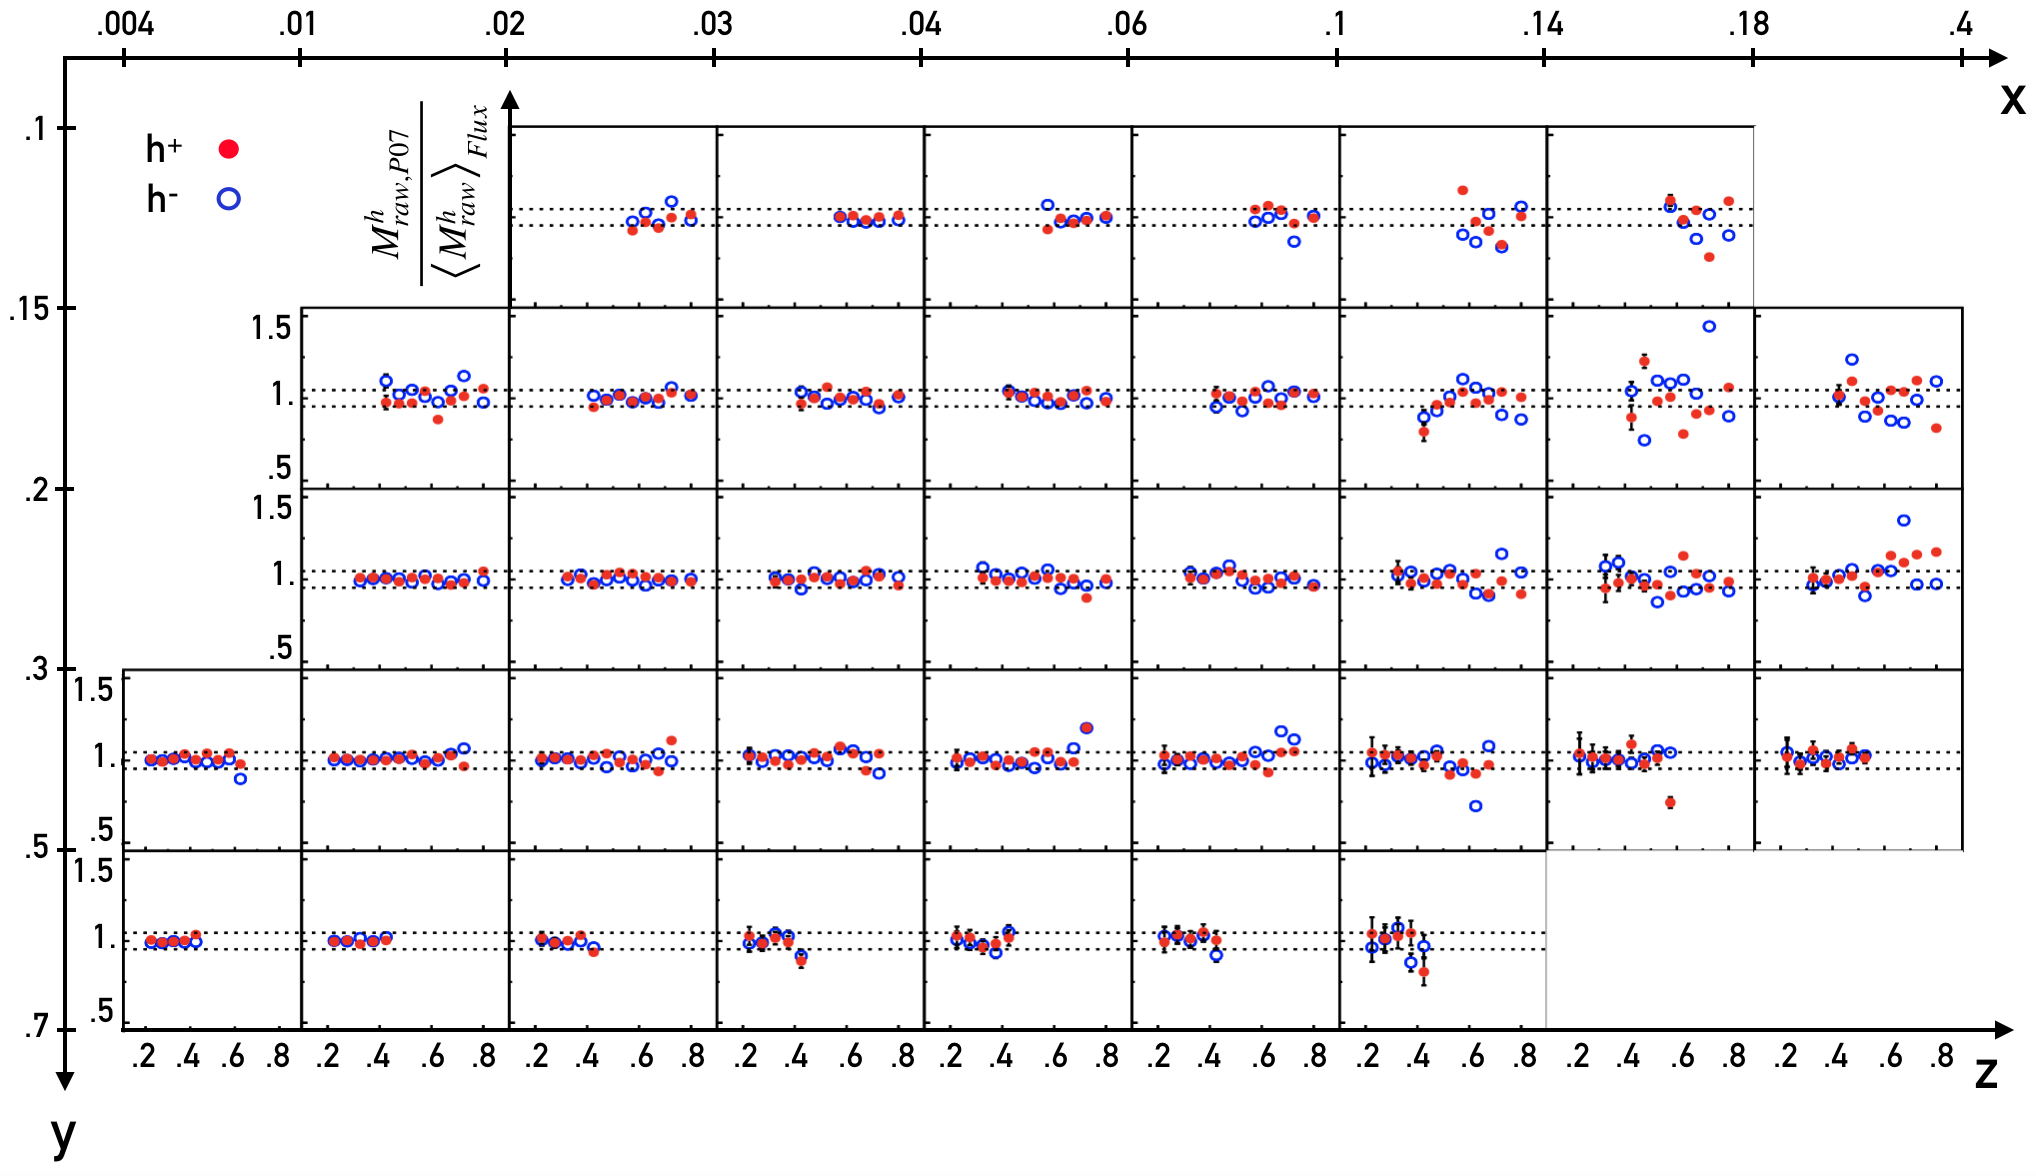
\includegraphics[scale=0.7]{./gfx/SysTimeMult.png}
	\caption{Ratio of P$07$ raw multiplicities over the raw multiplicities of all periods averaged over flux versus $z$. The red markers are for positive hadrons and the blue markers for negative hadrons. Each column corresponds to a given $x$ bin and each row to a given $y$ bin.}
	\label{pic:hMultTime}
\end{sidewaysfigure}

%------------------------------------------------

\subsection{Systematic uncertainty associated to the stability of data over beam charge}

The data samples used in the analysis were recorded with two different beam charges. Using the same method than in the previous subsection, a comparison was made for both beam charges and the results were compatible within statistical fluctuations. Consequently, no systematic error will be assigned for the beam charge change.

%------------------------------------------------

\subsection{Systematic uncertainty associated to the rescue procedure}


The rescue procedure might introduce background into the selected hadron sample. By applying quality cuts and the requirements at the RICH entrance, this contribution is negligible. Consequently, no systematic uncertainty is assigned for this rescue procedure.

%------------------------------------------------

\subsection{Systematic uncertainty associated to Monte Carlo sample : DJANGOH dependence}

To determine the acceptance dependence with the physical model chosen, different PDF sets were used to generate different MC samples. Moreover different JETSET parameters were also used \cite{PDFsys}. For each sample the acceptance is calculated and the hadron multiplicities are corrected with each acceptance. The systematic uncertainty of the acceptance, considering two acceptances $A^h$ and $A'^h$, is estimed in each kinematic bin ($x$,$y$,$z$) :

\begin{equation}
  \sigma^{A^h}_{syst} = \left| \frac{\left(\frac{A'^h}{A^h}-1 \right)M^h_{corr,acc}}{A^h} \right|
\end{equation}

The value of $\sigma^{A^h}_{syst}$ was found to be of $\sim$ $5$\%.

To study the quality of the spectrometer description the target was split into four different parts. For the comparison the multiplicities were integrated over $z$ and averaged over $y$ and then compared for each part of the target (Fig.~\ref{pic:Zvertexsum}). From this comparison, a conservative systematic error of $\sim$ $5$\% was derived.

\begin{figure}[!h]
  \centering
	\subfloat[]{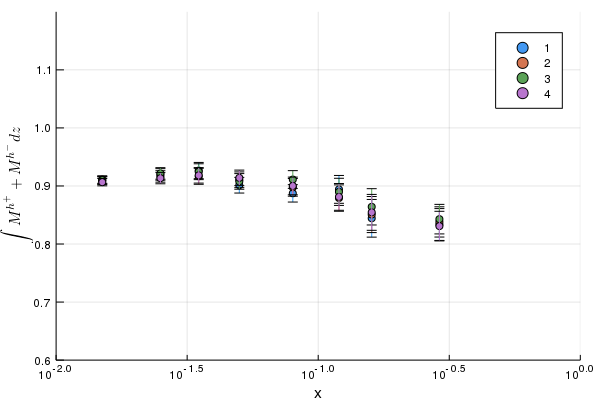
\includegraphics[scale=0.5]{./gfx/SumVertex.png}} \\
  \subfloat[]{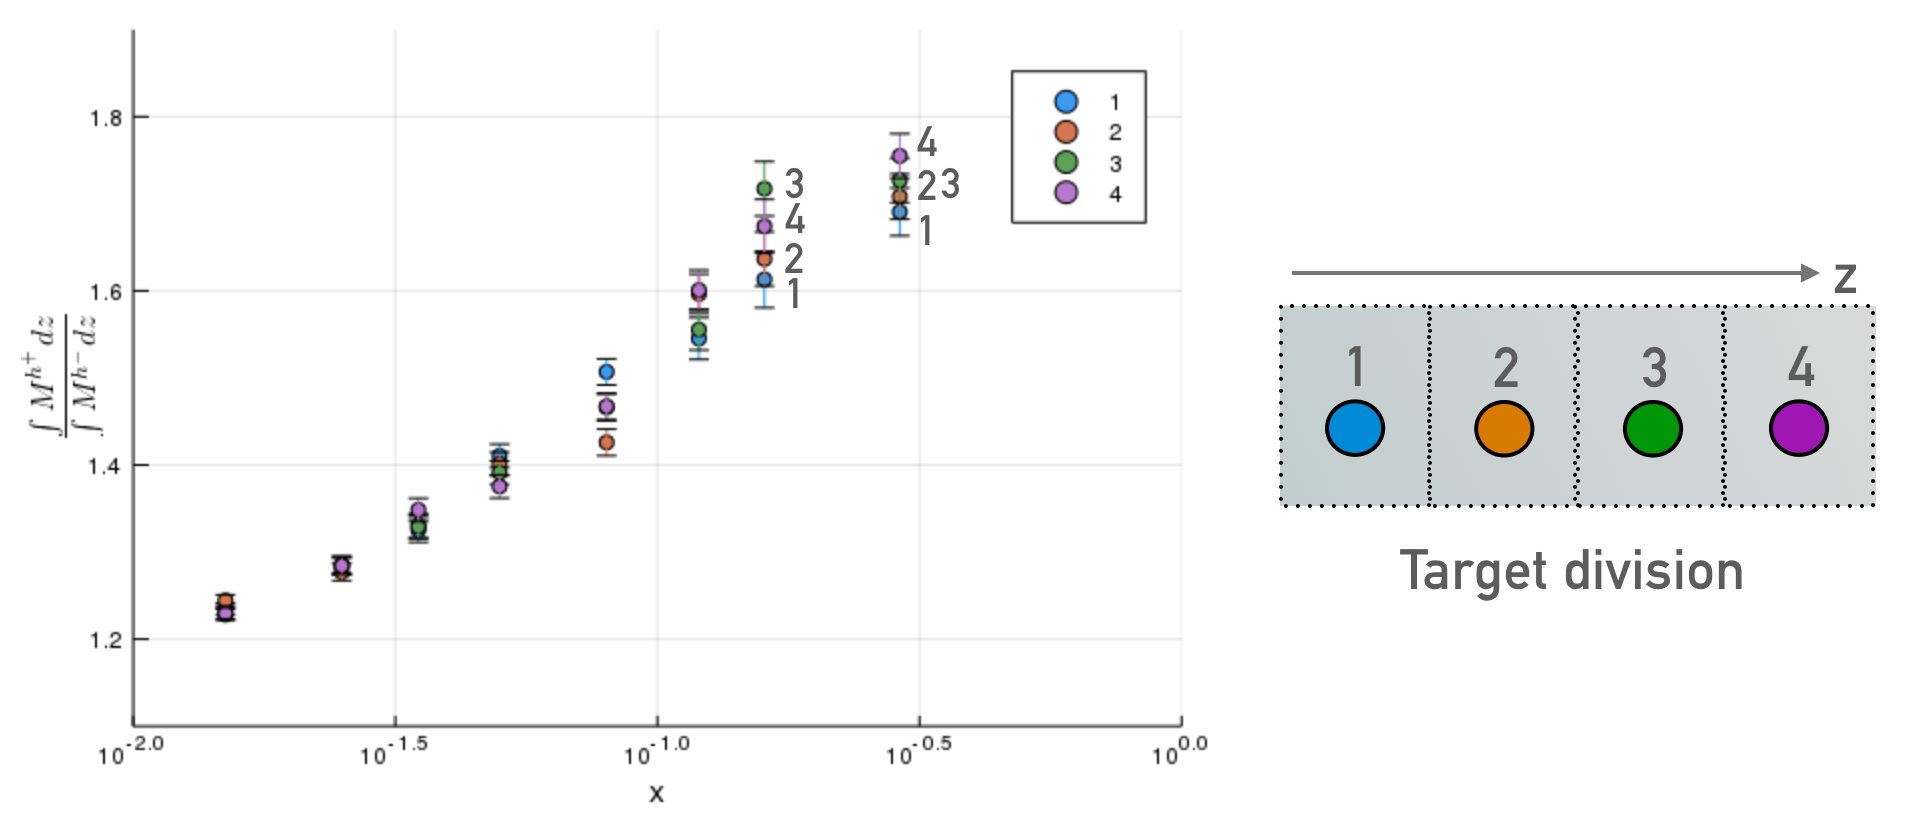
\includegraphics[scale=0.5]{./gfx/RatioVertex.png}}
	\caption{Comparison of the multiplicity sum (a) and ratio (b) for unidentified hadrons for different target slices.}
	\label{pic:Zvertexsum}
\end{figure}

In the end, a total systematic uncertainty of $\sim$ $10$\% is assumed for the acceptance.

%------------------------------------------------

\subsection{Systematic uncertainty associated to the diffractive vector meson correction}

In HEPGEN, the cross section for exclusive vector meson production is given by the GPD model of Goloskokov and Kroll. The theoretical uncertainty on the predicted cross section close to COMPASS kinematics is around $30$\% \cite{Goloskokov}. Propagating this uncertainty leads to a maximum relative uncertainty below $6$\%.

%----------------------------------------------------------------------------------------

\section{Charged hadron multiplicities ($h^{\pm}$,$\pi^{\pm}$,$K^{\pm}$,$p/\bar{p}$)}

The final results for the multiplicities are obtained as :
%
\begin{equation}
  	M^h_{Final}(x,y,z) = M^h_{raw}(x,y,z)\frac{\eta^h(x,y,z)}{A^h(x,y,z)}B^h(x,y,z),
\end{equation}
%
including all corrections described in the previous section.
The $x$,$y$ and $z$ binning is given in Table~\ref{tab:kinbinning}. $A^h$ corresponds to the acceptance correction (Section~\ref{sec:Acc}), $\eta^h$ to the radiative correction factor (Section~\ref{sec:rcf}) and $B^h$ to the diffractive vector meson correction factor (Section~\ref{sec:DVMf}). The statistical error propagation is performed in all ($x,y,z$) bins assuming that all corrections are independent :
%
\begin{equation}
\begin{split}
		E^2_{Final} = \bigg( \frac{\eta^h \cdot B^h}{A^h} \bigg)^2 E^2_{raw} + \bigg(\frac{\eta^h \cdot B^h \cdot M^h_{raw}}{Acc^2} \bigg)^2 E^2_{Acc} \\
		+ \bigg(\frac{\eta^h \cdot M^h_{raw}}{Acc} \bigg)^2 E^2_{VM} + \bigg(\frac{B^h \cdot M^h_{raw}}{Acc} \bigg)^2 E^2_{RC}.
\end{split}
\end{equation}
%
The corresponding systematic uncertainties from the different sources are added quadratically. The largest contribution in most bins comes from the systematic uncertainty of the acceptance.

\subsection{Final charged hadron multiplicities}

The 300 data points for each of the charged hadron multiplicities $M^{h^{\pm}}$ are shown in Figs.~\ref{pic:mhp} to \ref{pic:mpm} as a function of $z$, in bins of $x$ and staggered vertically with $y$. A strong $z$ dependence is observed for all ($x$,$y$) bins as well as a small dependence with $x$. The $Q^2$ values are in the range $1$ to $30$ (GeV/$c$)$^2$. The statistical uncertainties are too small to be visible in almost all kinematic bins. The bands at the bottom of each $x$ bin panel are the systematic errors for the bin $0.3$ $< y <$ $0.5$ (bin that covers the largest $z$ range). They are very similar but not shown for the other $y$ bins.

\begin{figure}[!h]
  \centering
	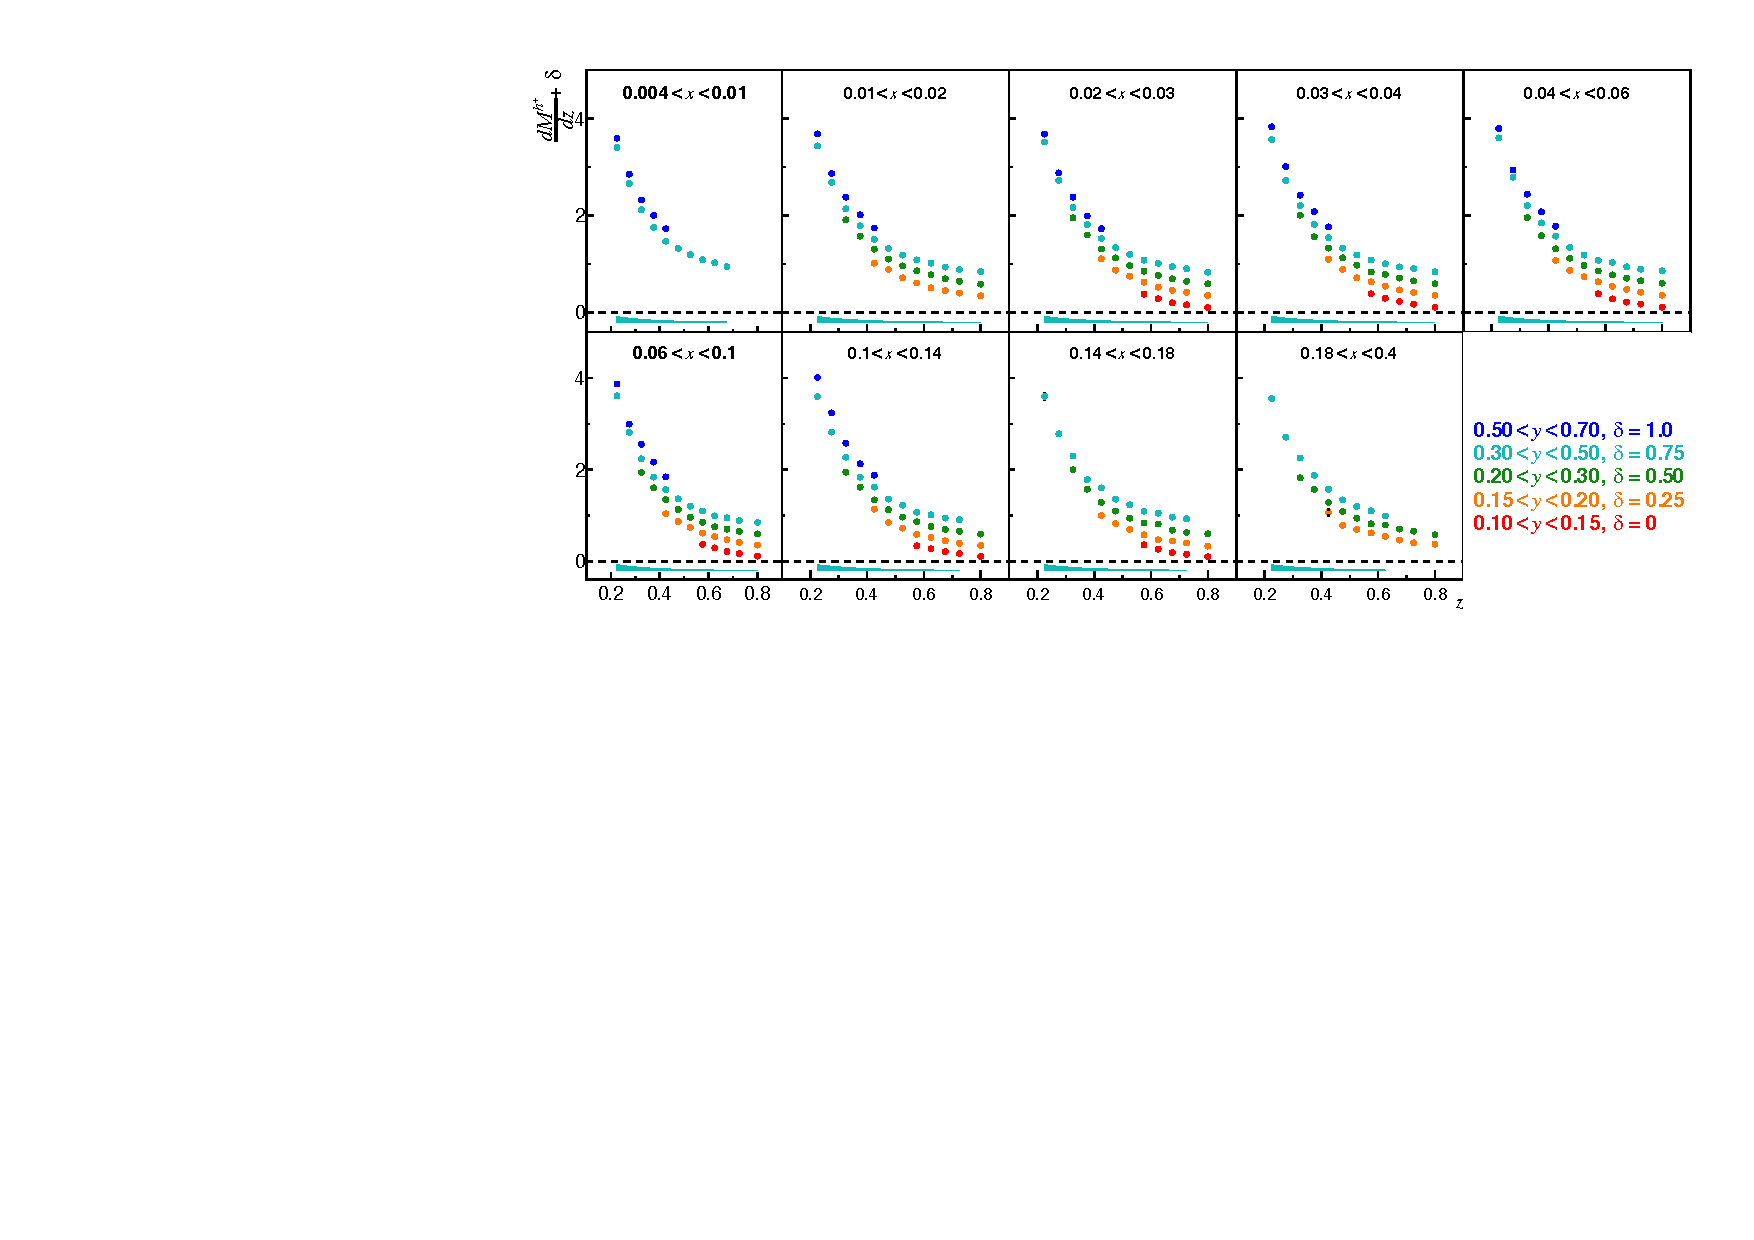
\includegraphics[scale=0.85]{./gfx/hp.pdf}
	\caption{Unidentified positive hadron multiplicities (with all corrections) as a function of $z$ in bins of $x$ staggered vertically with $y$.}
	\label{pic:mhp}
\end{figure}

\newpage

\begin{figure}[!h]
  \centering
	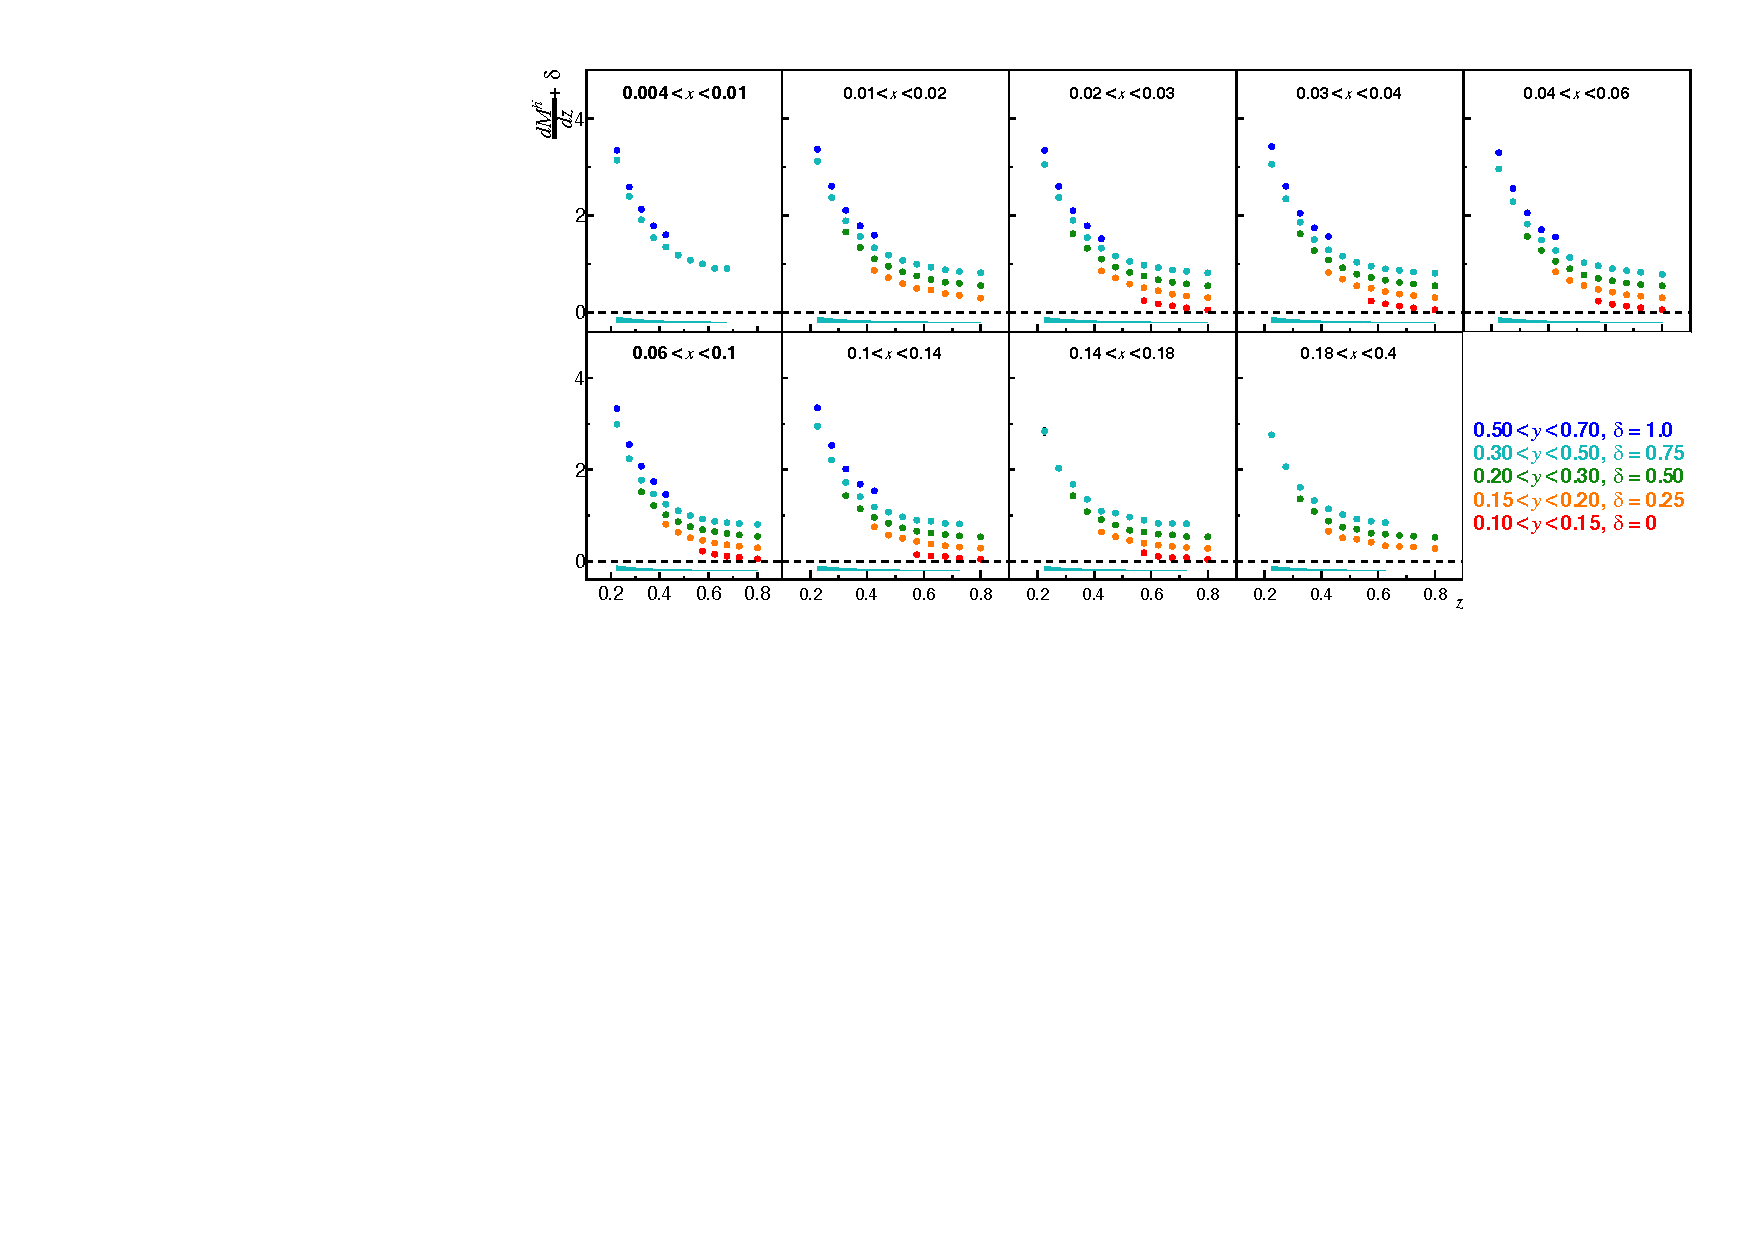
\includegraphics[scale=0.85]{./gfx/hm.pdf}
	\caption{Unidentified positive hadron multiplicities (with all corrections) as a function of $z$ in bins of $x$ staggered vertically with $y$.}
	\label{pic:mhm}
\end{figure}

\begin{figure}[!h]
  \centering
	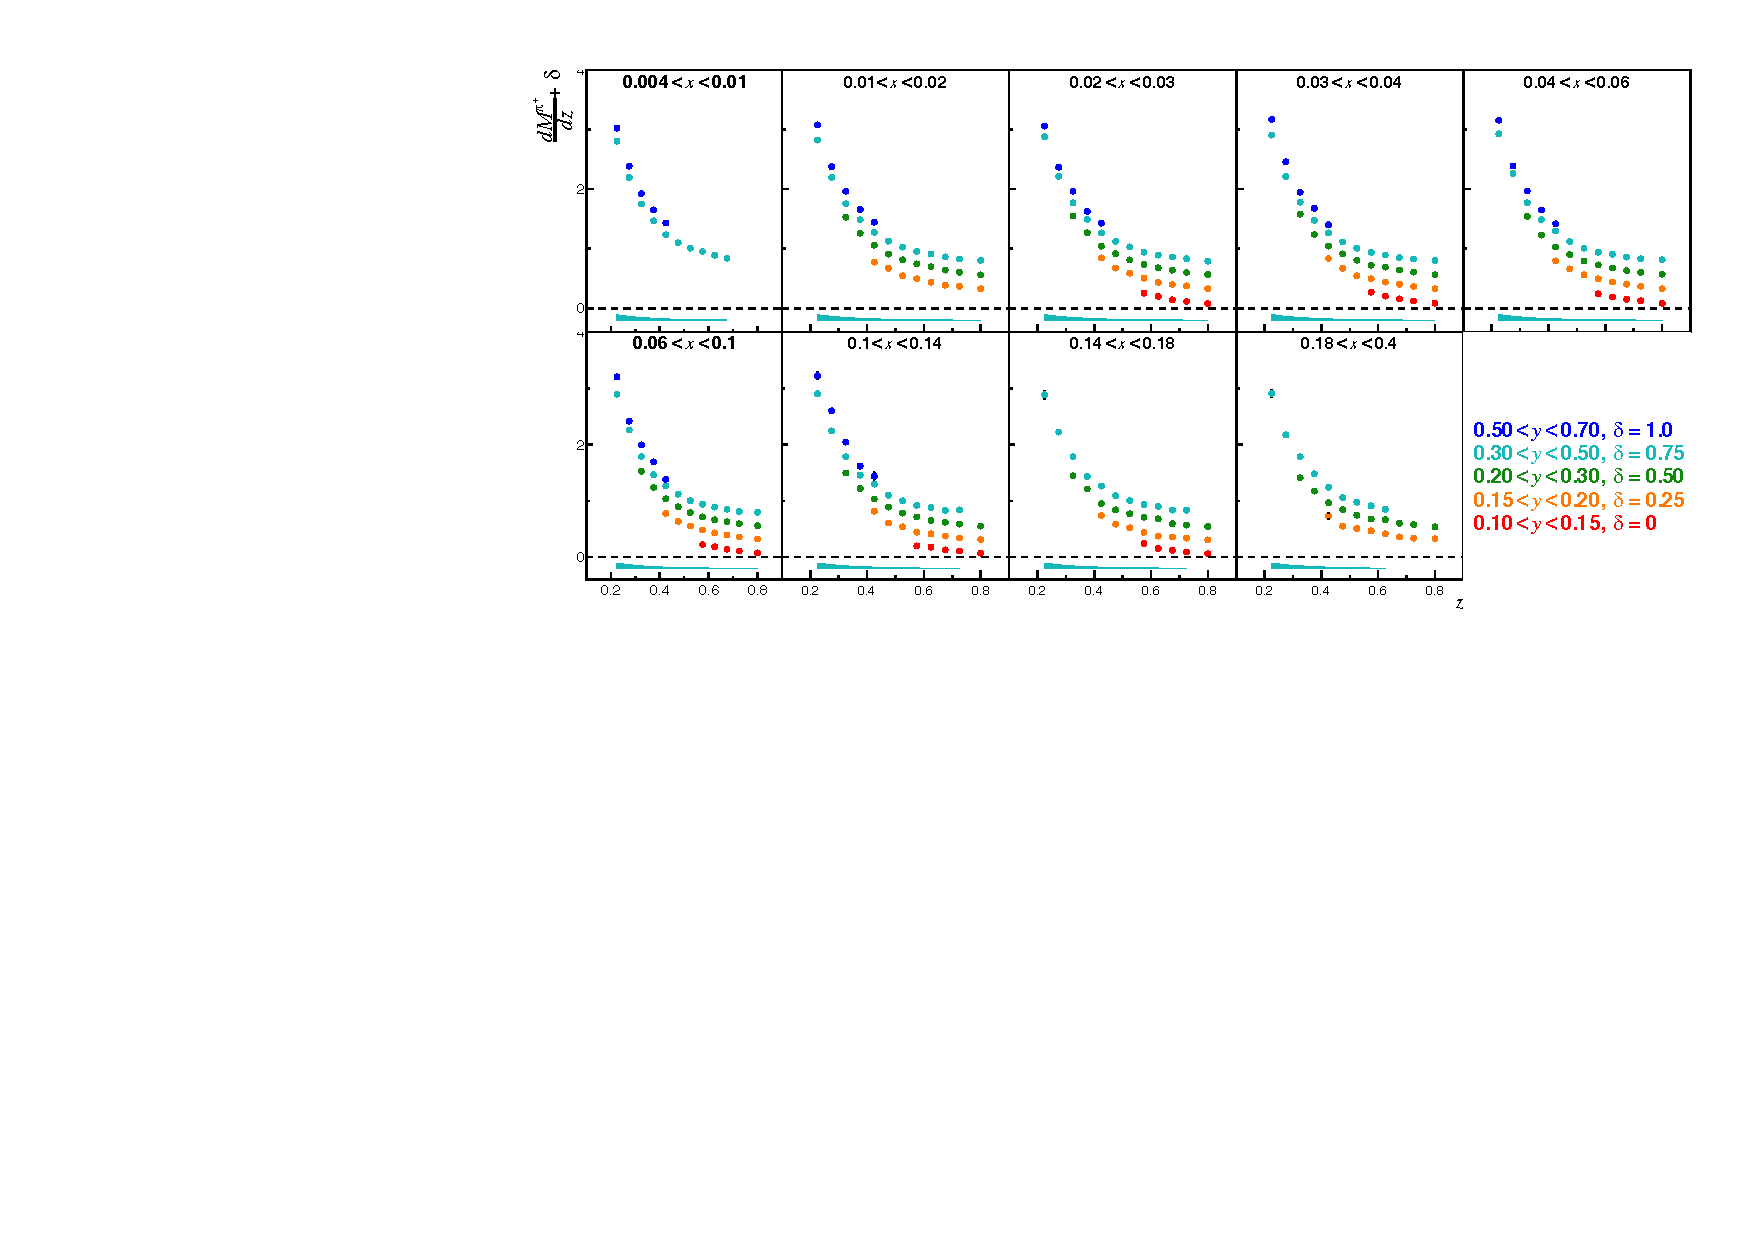
\includegraphics[scale=0.85]{./gfx/pip.pdf}
	\caption{Positive pion multiplicities (with all corrections) as a function of $z$ in bins of $x$, staggered vertically with $y$.}
	\label{pic:mpip}
\end{figure}

\newpage

\begin{figure}[!h]
  \centering
	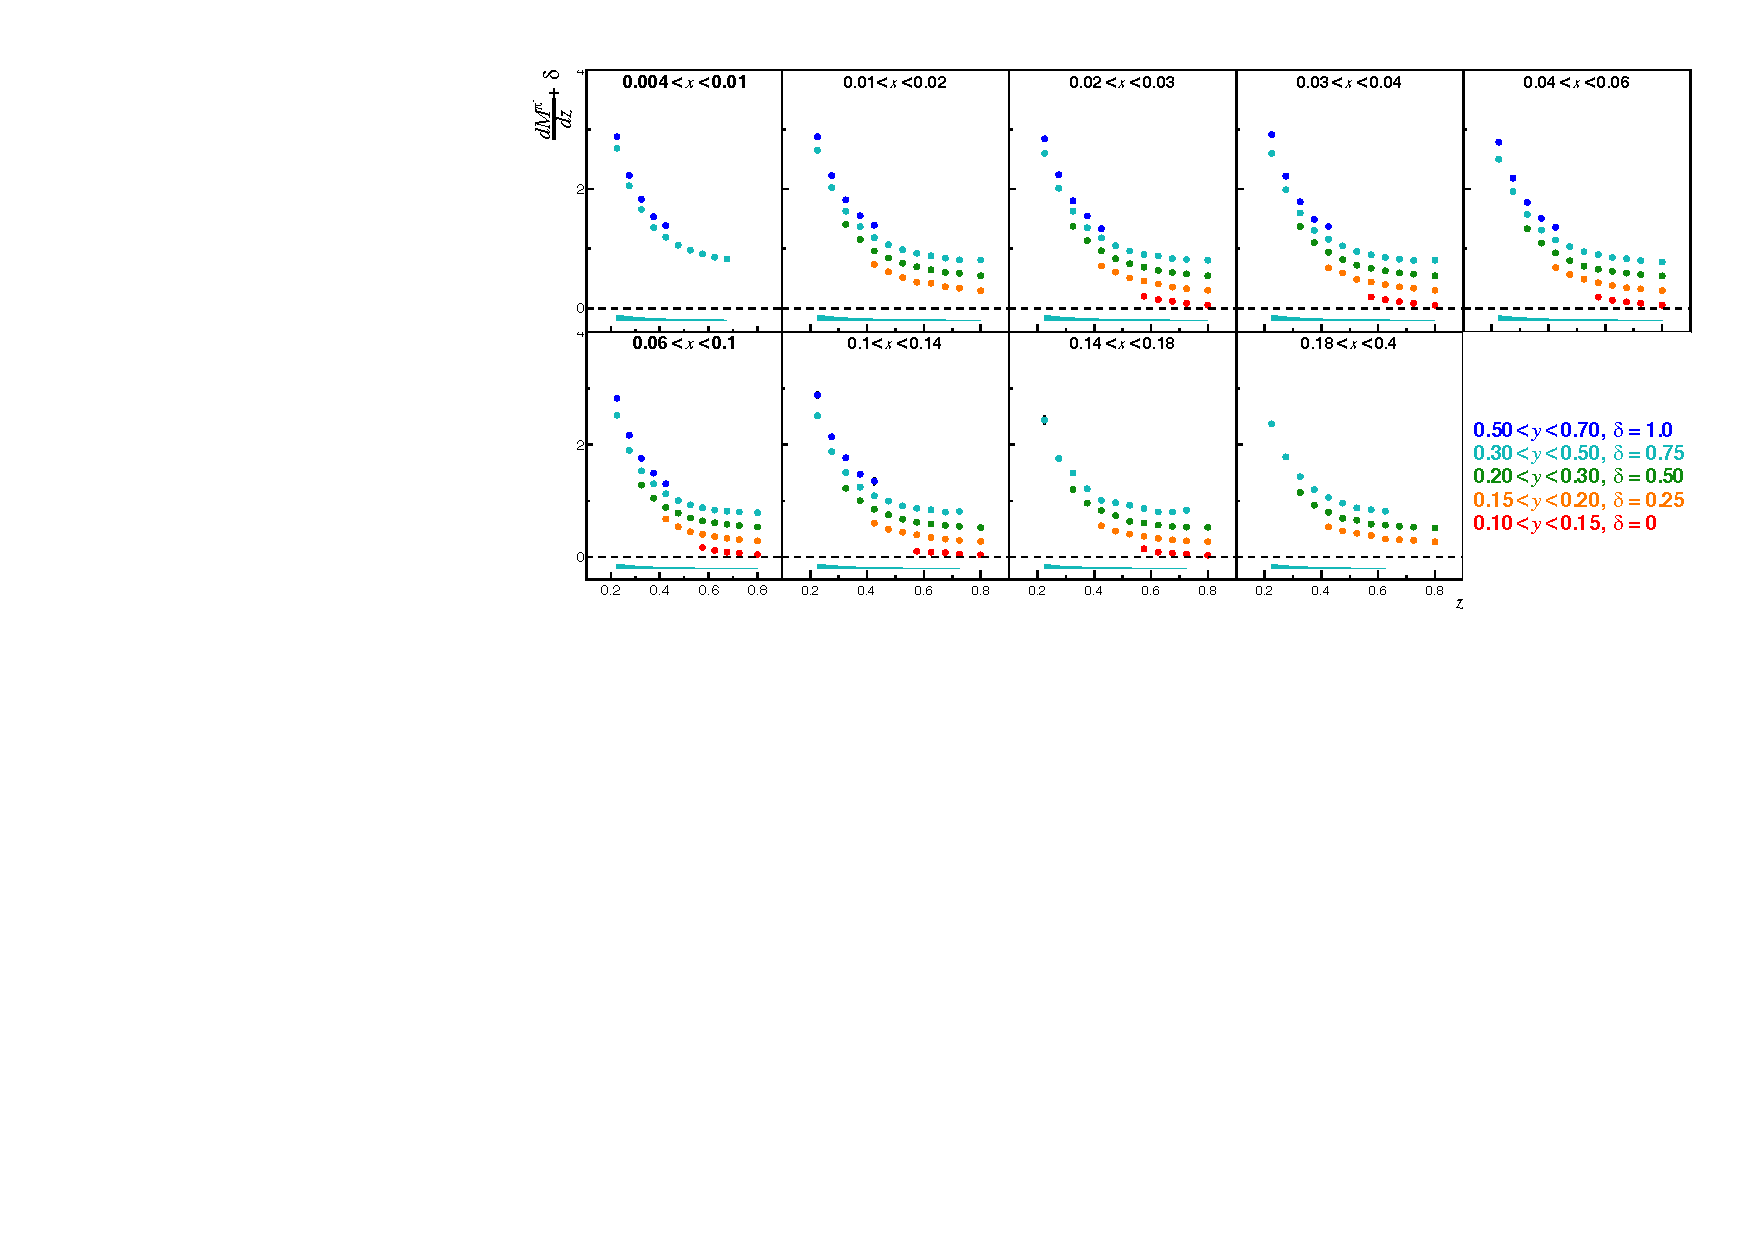
\includegraphics[scale=0.85]{./gfx/pim.pdf}
	\caption{Negative pion multiplicities (with all corrections) as a function of $z$ in bins of $x$, staggered vertically with $y$.}
	\label{pic:mpim}
\end{figure}

\begin{figure}[!h]
  \centering
	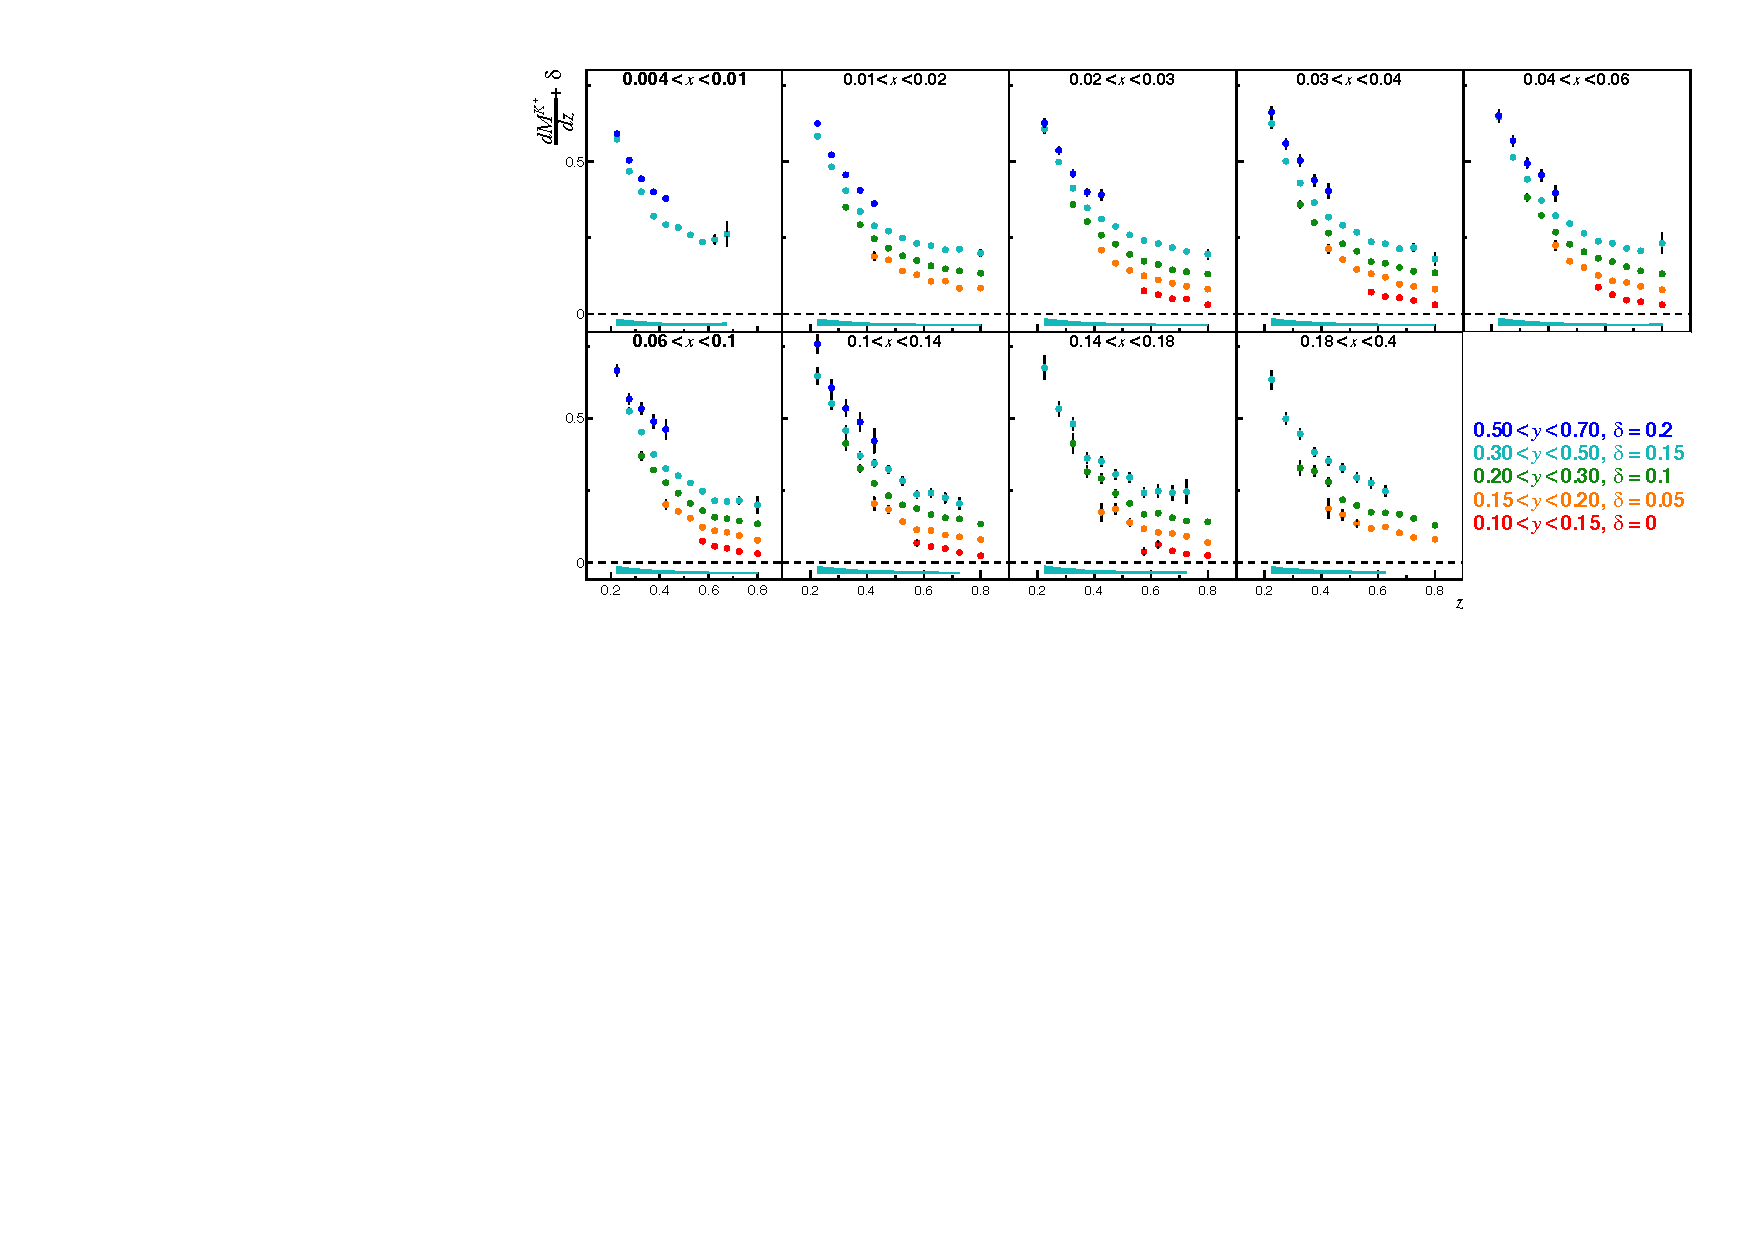
\includegraphics[scale=0.85]{./gfx/Kp.pdf}
	\caption{Positive kaon multiplicities (with all corrections) as a function of $z$ in bins of $x$, staggered vertically with $y$.}
	\label{pic:mkp}
\end{figure}

\newpage

\begin{figure}[!h]
  \centering
	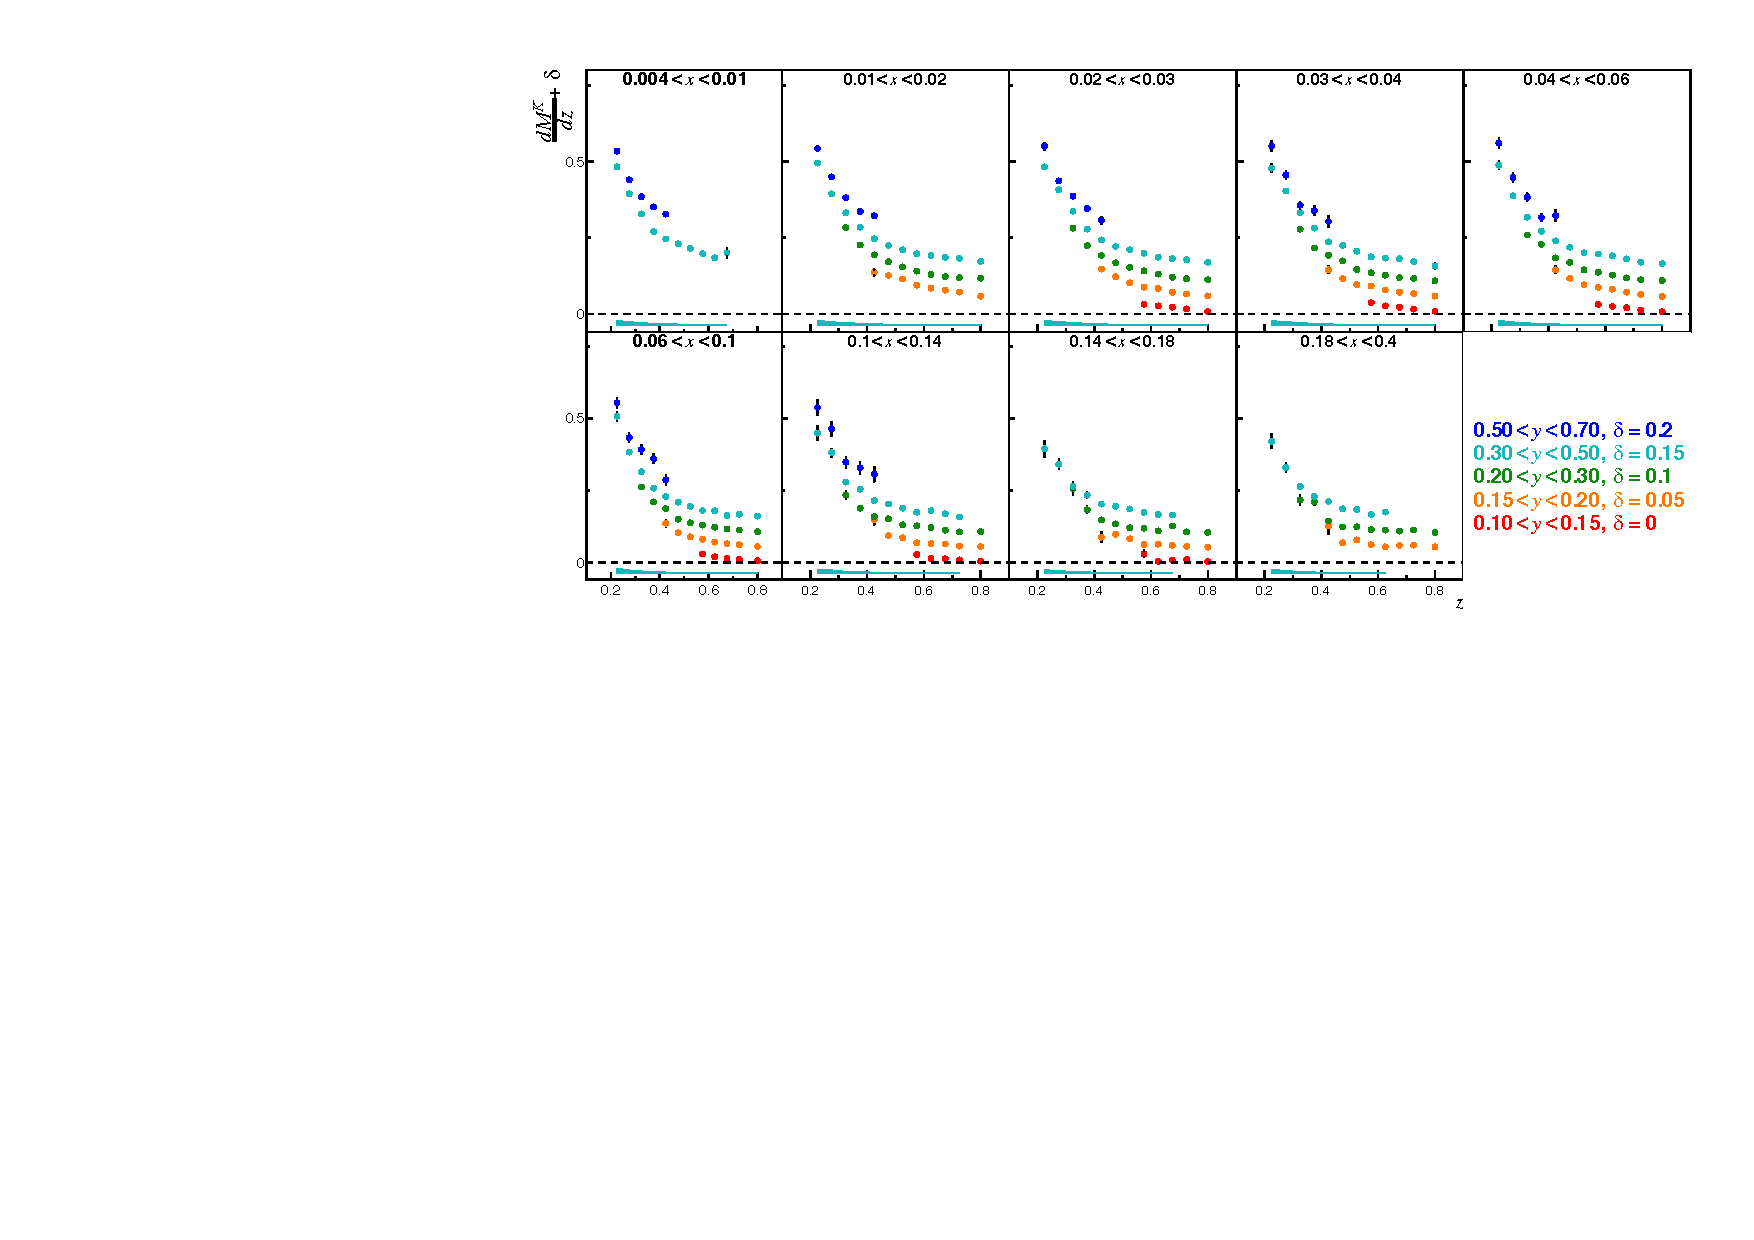
\includegraphics[scale=0.85]{./gfx/Km.pdf}
	\caption{Negative kaon multiplicities (with all corrections) as a function of $z$ in bins of $x$, staggered vertically with $y$.}
	\label{pic:mkm}
\end{figure}

\begin{figure}[!h]
  \centering
	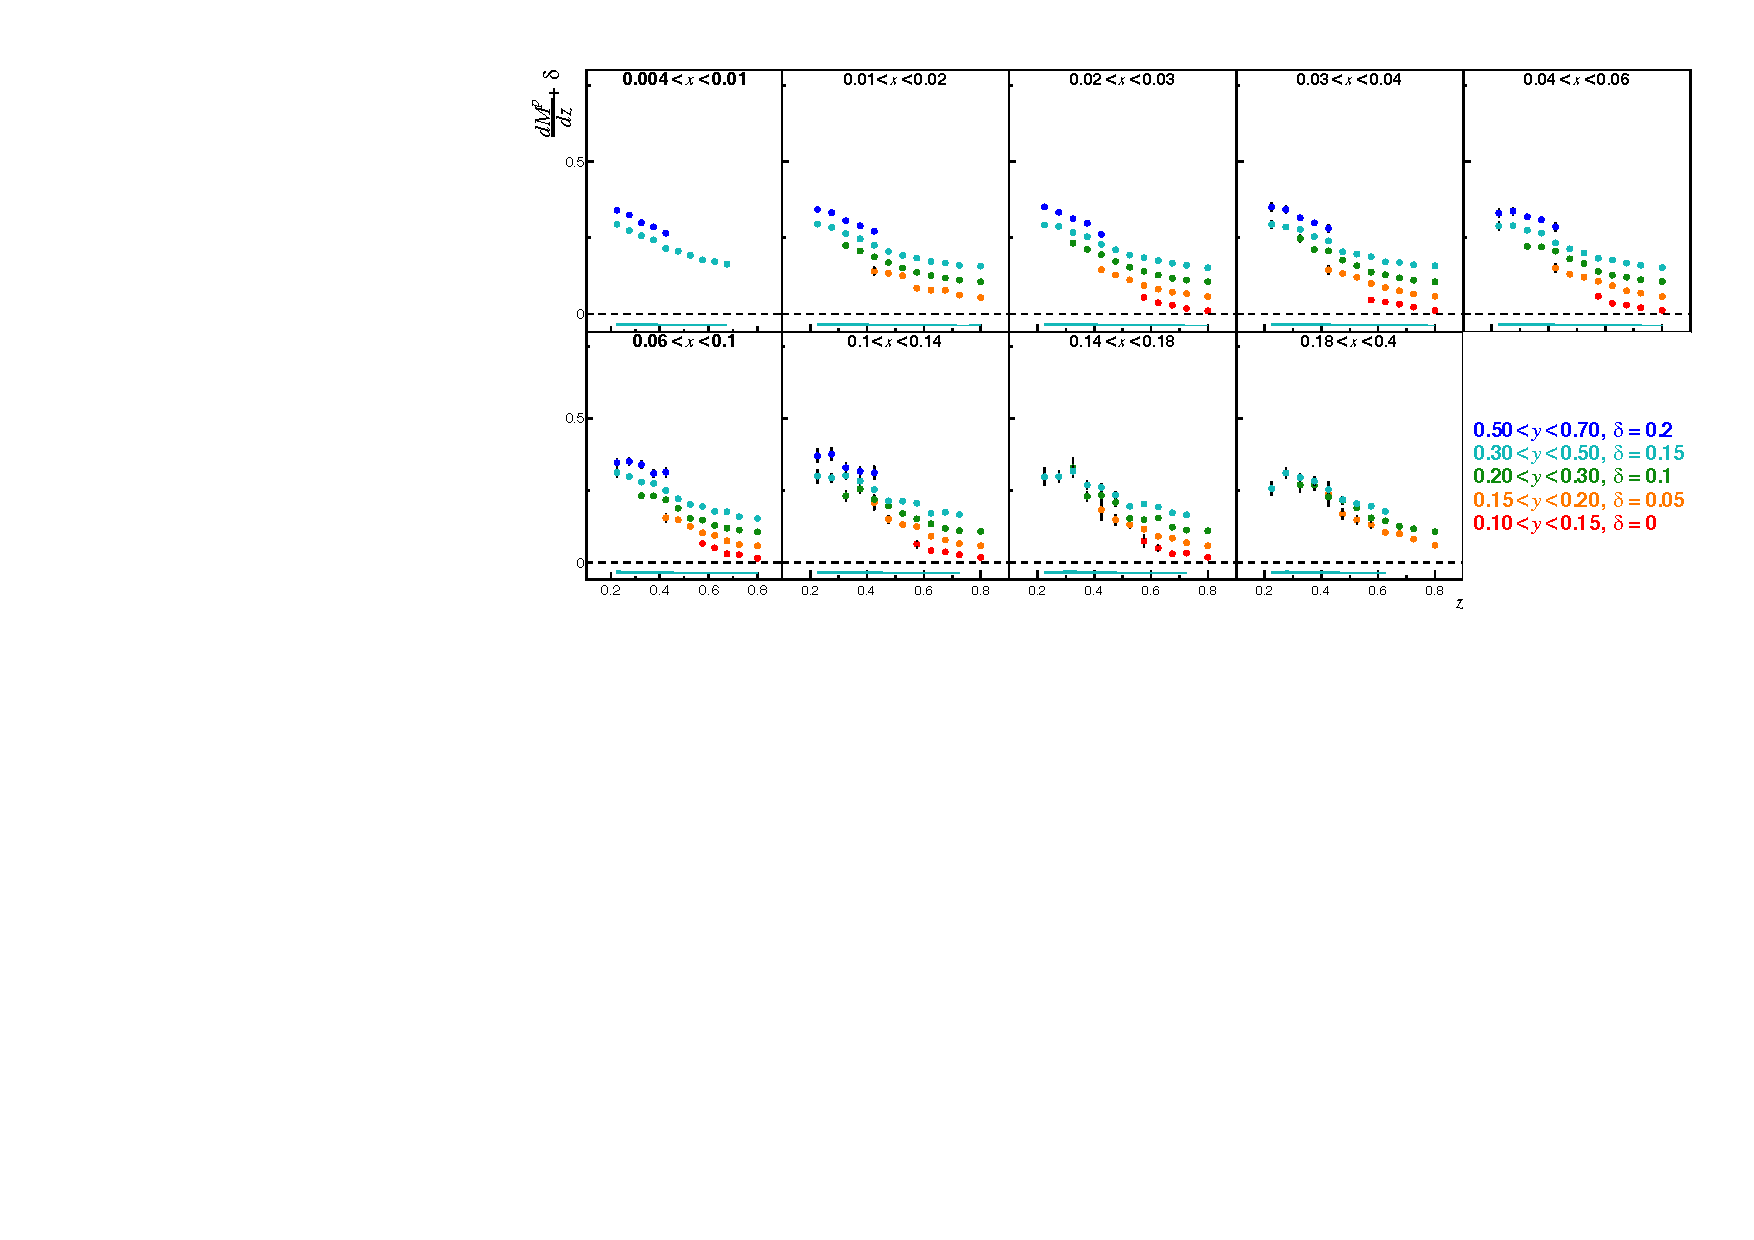
\includegraphics[scale=0.85]{./gfx/pp.pdf}
	\caption{Proton multiplicities (with all corrections) as a function of $z$ in bins of $x$, staggered vertically with $y$.}
	\label{pic:mpp}
\end{figure}

\newpage

\begin{figure}[!h]
  \centering
	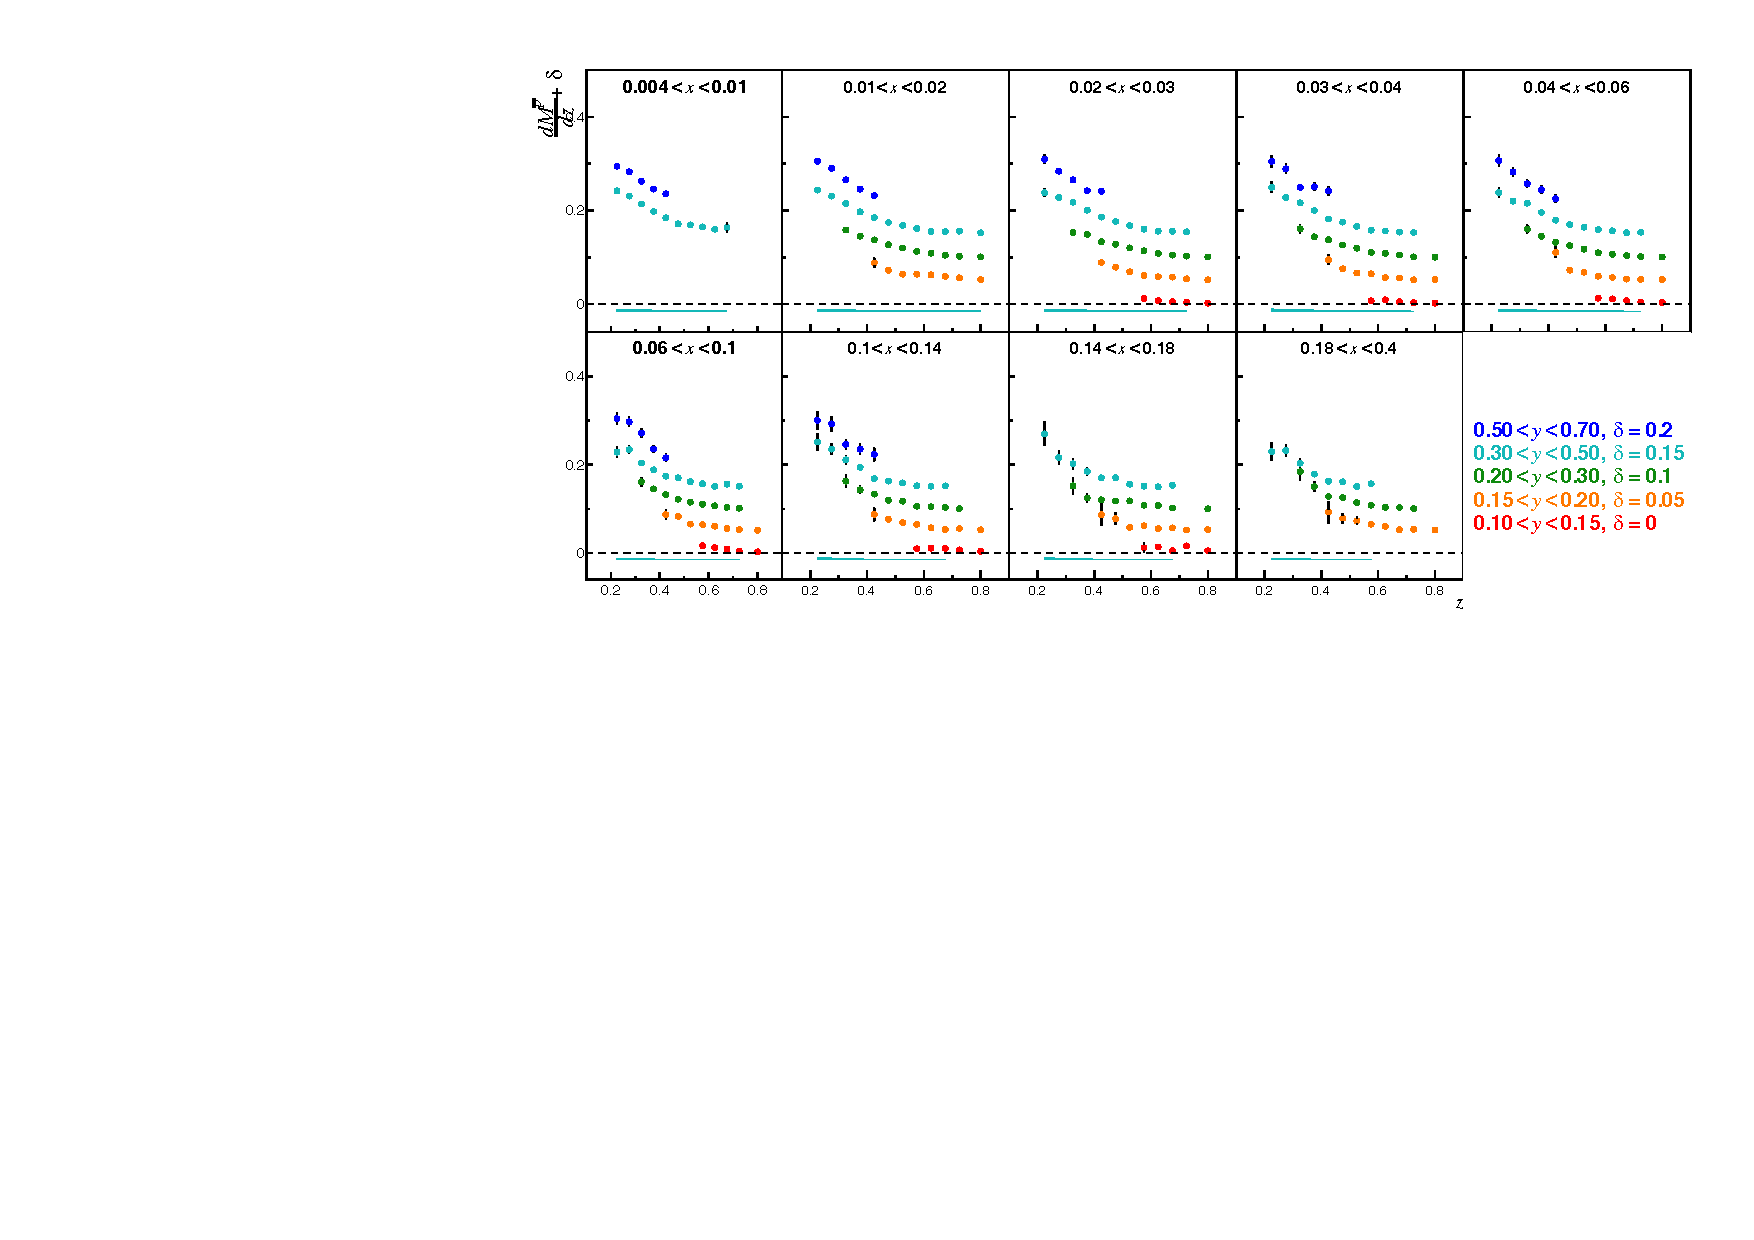
\includegraphics[scale=0.85]{./gfx/pm.pdf}
	\caption{Antiproton multiplicities (with all corrections) as a function of $z$ in bins of $x$, staggered vertically with $y$.}
	\label{pic:mpm}
\end{figure}

When removing the $y$ staggering on the previous results, one can see that the results from different $y$ bins agree very well in the overlap region (Fig.~\ref{pic:mhnoy}). That means that our multiplicities results have no $y$ dependence and can then be averaged over $y$, using the square of the statistical error as weight.

\begin{figure}[!h]
  \centering
	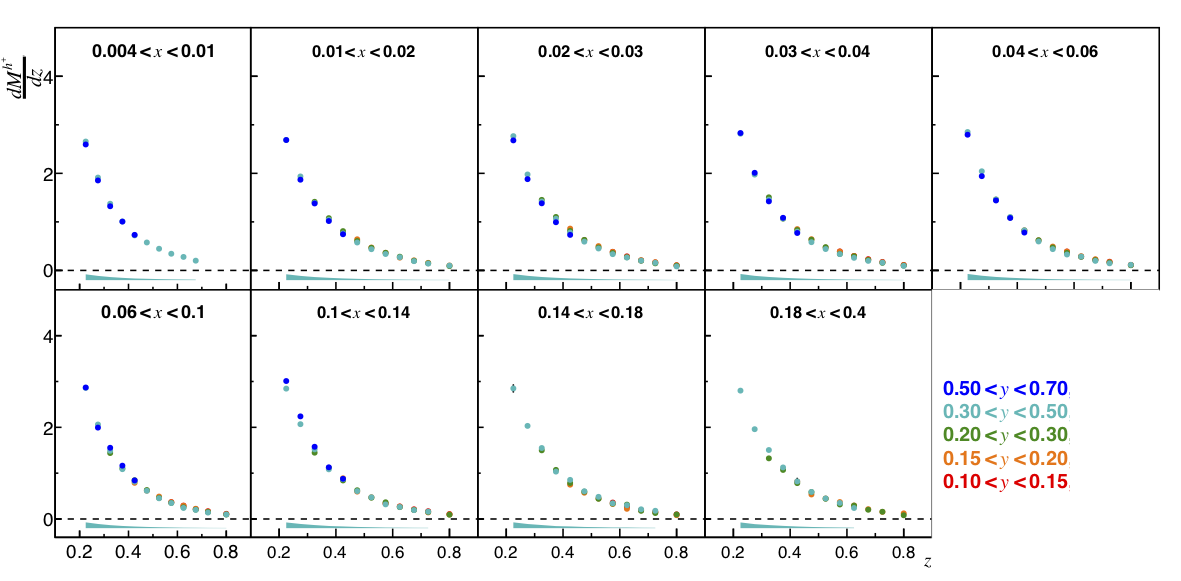
\includegraphics[scale=0.85]{./gfx/hnoystag.png}
	\caption{Unidentified positive hadron multiplicities (with all corrections) as a function of $z$ in bins of $x$. The vertical staggering with $y$ has been suppressed showing that the different $y$ bins do overlap.}
	\label{pic:mhnoy}
\end{figure}

Then the multiplicities are shown as a function of $z$ and in bins of $x$ in Figs.~\ref{pic:mhyavg} to \ref{pic:mpyavg}. An asymmetry between all positive and negative charged hadrons is observed, increasing with $x$. The size of the asymmetry depends on the hadron species. Having more $\pi^+$ than $\pi^-$ is due to the fact there is a dominant $u$ quark distribution in the target but the asymmetry is smaller than for hadrons. The strong asymmetry between $K^+$ and $K^-$ is due to the fact there is a dominant valence $u$ quark distribution in the target, whereas producing leading  $K^-$ is only possible with sea quarks. The same statement can be made for proton and antiproton.

\begin{figure}[!h]
  \centering
	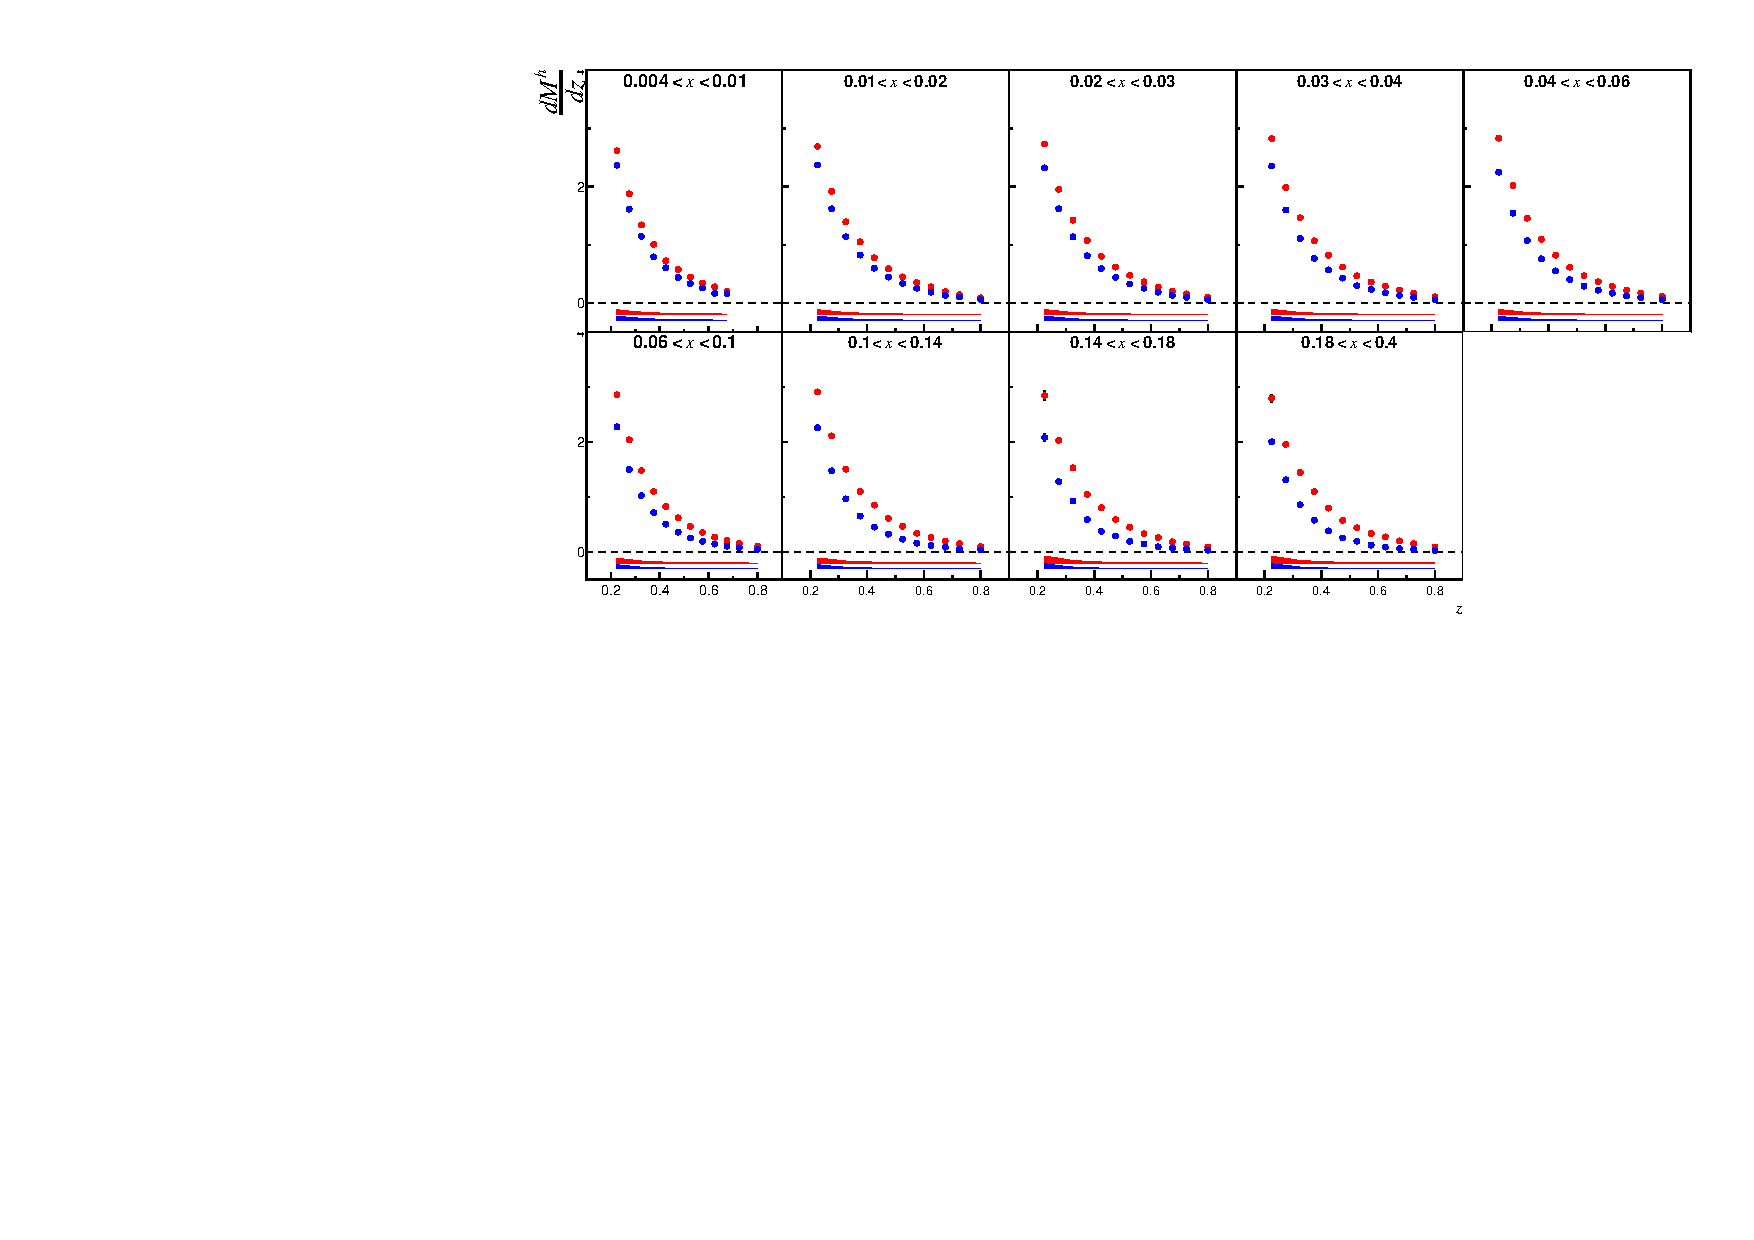
\includegraphics[scale=0.85]{./gfx/hyavg.pdf}
	\caption{Unidentified positive (red) and negative (blue) hadron multiplicities (with all corrections) averaged over $y$ as a function of $z$ in bins of $x$.}
	\label{pic:mhyavg}
\end{figure}

\begin{figure}[!h]
  \centering
	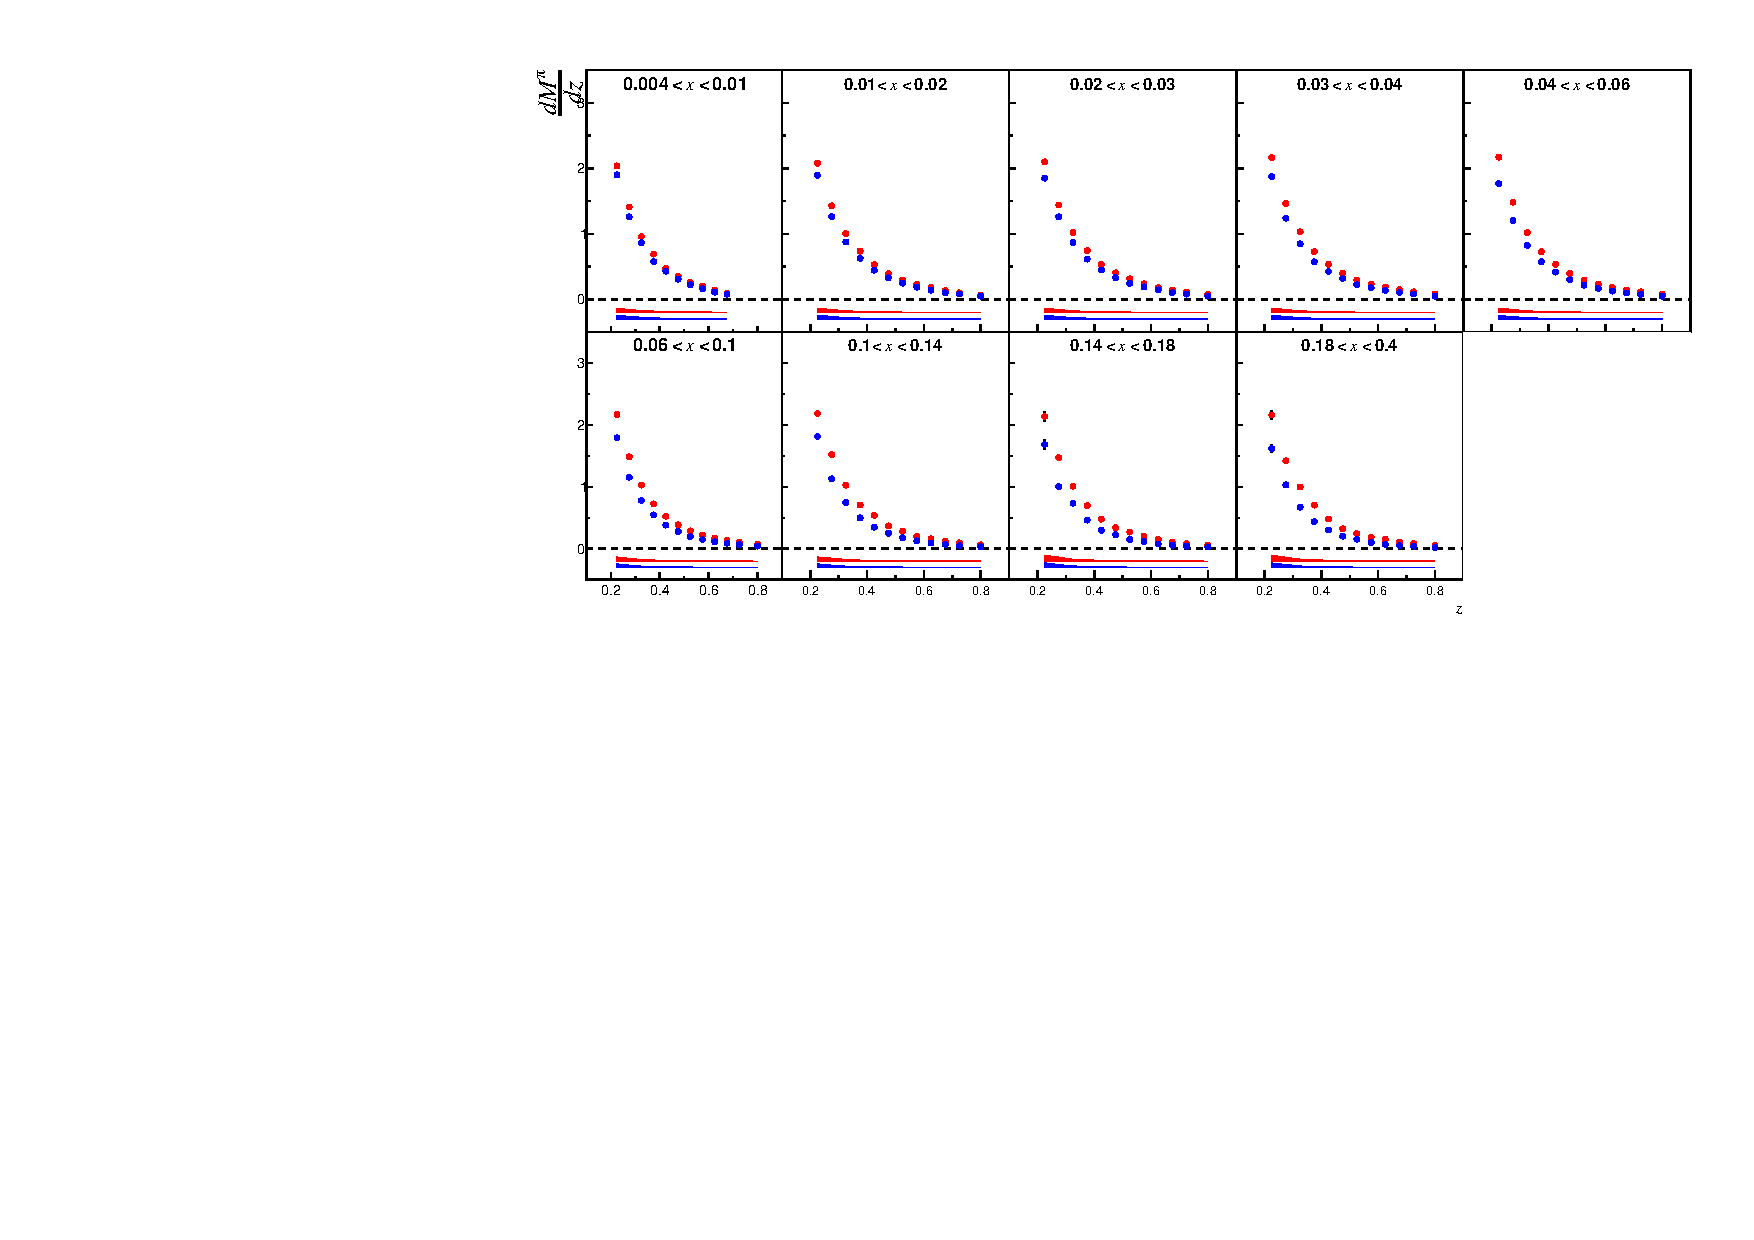
\includegraphics[scale=0.85]{./gfx/piyavg.pdf}
	\caption{Positive (red) and negative (blue) pion multiplicities (with all corrections) averaged over $y$ as a function of $z$ in bins of $x$.}
	\label{pic:mpiyavg}
\end{figure}

\newpage

\begin{figure}[!h]
  \centering
	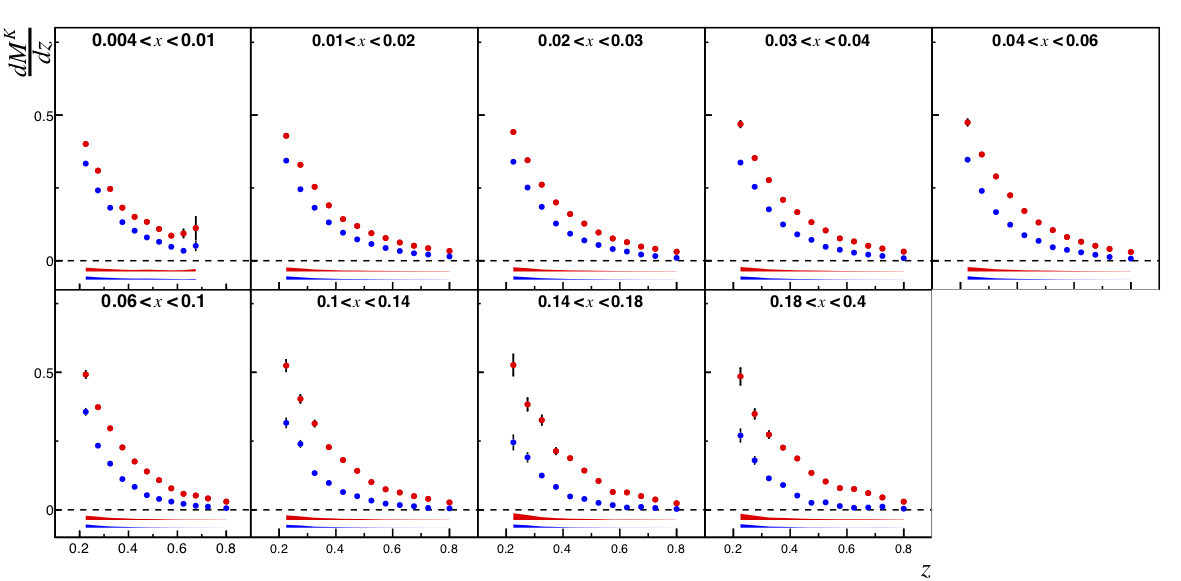
\includegraphics[scale=0.85]{./gfx/Kyavg.png}
	\caption{Positive (red) and negative (blue) kaon multiplicities (with all corrections) averaged over $y$ as a function of $z$ in bins of $x$.}
	\label{pic:mkyavg}
\end{figure}

\begin{figure}[!h]
  \centering
	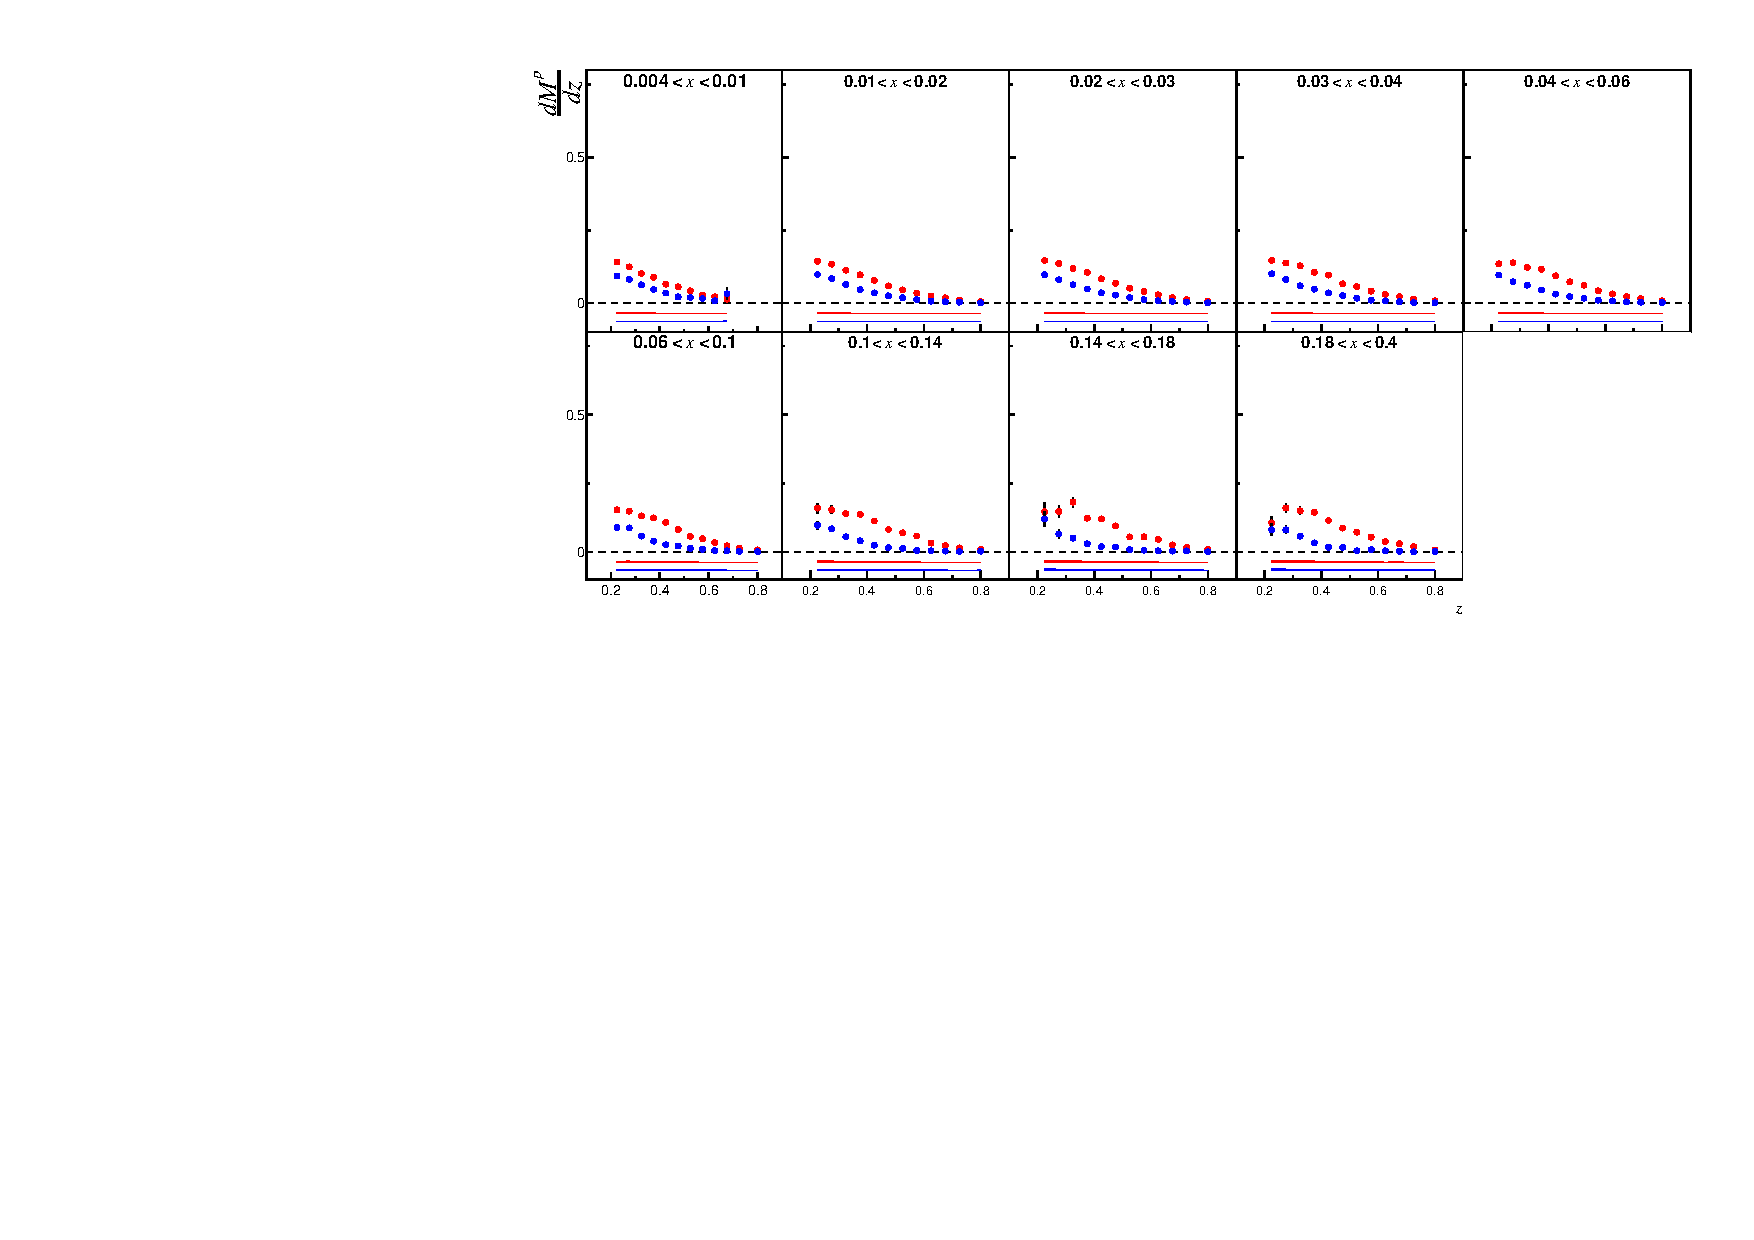
\includegraphics[scale=0.85]{./gfx/pyavg.pdf}
	\caption{Proton (red) and antiproton (blue) multiplicities (with all corrections) averaged over $y$ as a function of $z$ in bins of $x$.}
	\label{pic:mpyavg}
\end{figure}

\newpage

\section{Ratio and sum of charged hadron multiplicities}

From the $y$-averaged multiplicities, we can still integrate on $z$. This allows us to have an idea of the underlying physics as some limiting cases for the $x$ dependence, when integrating over $z$, can be investigated. In addition it also allows us to compare our results with other experiments that have different binning in ($x,Q^2,z$). From the integration over $z$ only the 8 $x$ bins that have a sufficient $z$ coverage subsist. One interesting quantity to look at is the ratio of charged hadron multiplicities as with this quantity most of the systematics cancel by and large. The ratio is calculated as following :
%
\begin{equation}
  \frac{\mathscr{M}^{h^+}}{\mathscr{M}^{h^-}} = \frac{\int_{0.2}^{0.85} \langle M^{h^+} \rangle_y dz}{\int_{0.2}^{0.85} \langle M^{h^-} \rangle_y dz}.
\end{equation}
%
An alternative approach is to look at the sum of charged hadron multiplicities $\mathscr{M}^{h^+}+\mathscr{M}^{h^-}$ in order to study multiplicities independent of the hadron charge. They are relevant quantity to compute as for some type of hadrons, the results between the multiplicities extracted on a proton target ($lH_2$, this analysis) and an isoscalar target ($^6LiD$, COMPASS published results \cite{COMPASS2006Pi,COMPASS2006K}) should be similar.

Hereafter the results from this analysis will be compared to COMPASS published results and HERMES published results \cite{HERMESMult}. HERMES has performed measurements of electron/positron of $27.6$ GeV scattering off proton and deuteron targets at DESY-HERA. The datasets selected for the comparison are the multiplicities of charged pions and charged kaons in bins of $x$ and $z$. The range of $z$ of these datasets is of [$0.1,1.1$] and the range in $y$ of [$0.1,0.85$].

\subsection{Ratio of charged hadron multiplicities}

In Figs.~\ref{pic:hratio} to \ref{pic:pratio}, the $\mathscr{M}^{h^+}/\mathscr{M}^{h^-}$ from COMPASS is depicted for a proton target (blue triangle) and for an isoscalar target (orange circles). The same ratio from HERMES is presented for a proton target (violet open squares) and a deuteron target (green open stars) for charged pions and charged kaons.

\begin{figure}[!h]
  \centering
	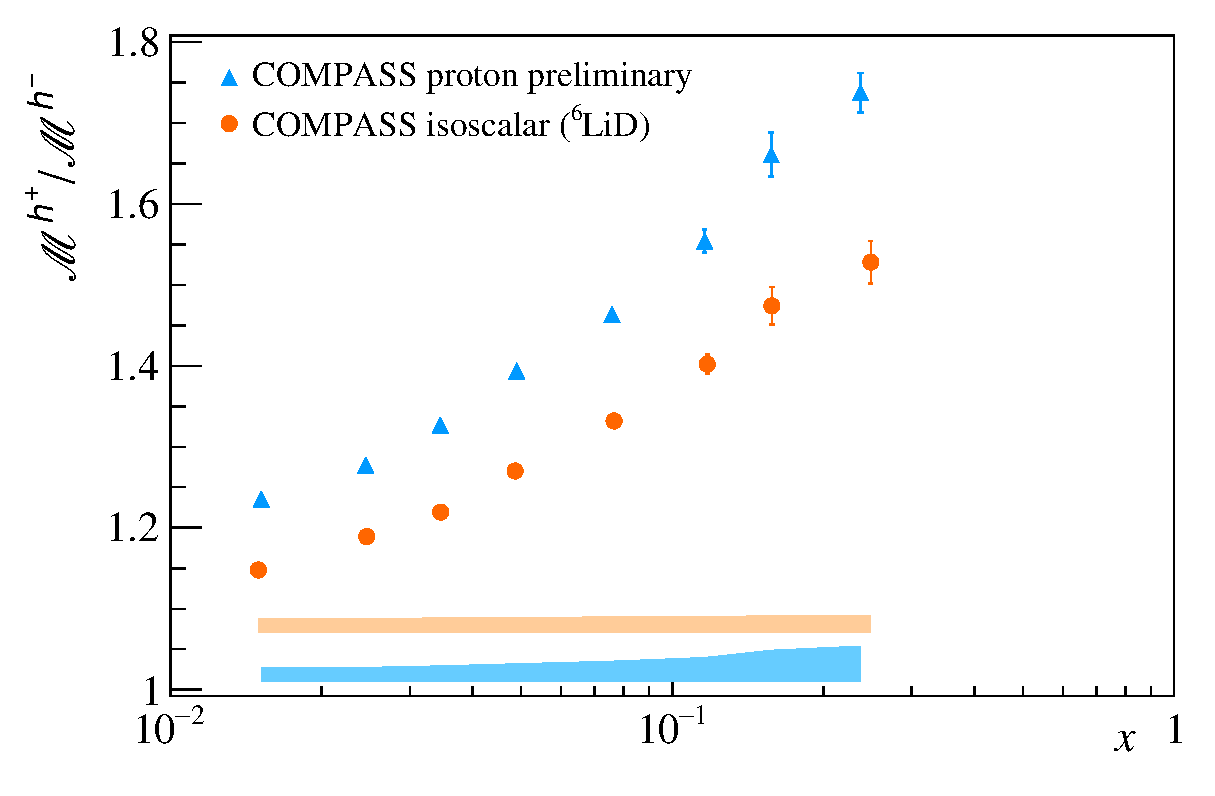
\includegraphics[scale=0.5]{./gfx/Mult_h_ratio.eps}
	\caption{Ratio of $\frac{\mathscr{M}^{h^+}}{\mathscr{M}^{h^-}}$ for a proton target (blue closed points) and an isoscalar target (orange closed points) (COMPASS data)}
	\label{pic:hratio}
\end{figure}

The ratio of unidentified charged hadron and pion multiplicity for a proton target should lie above COMPASS results on isoscalar target, the reason being the different quark mixture in the two targets (more $u$ in proton target thus higher $h+$/$h-$ ratio in proton than in isoscalar target). The difference is expected to be $\sim$$10-20$\%, as obtained here. The ratio of charged kaon multiplicity on proton target is expected to be larger than COMPASS results for isoscalar target by $\sim$$10$\%, as observed here. These expectations are obtained by evaluating the multiplicities for both targets with Eq.~\ref{eq:MFFPDF} taking DSS07 \cite{DSS07} LO fragmentation functions for hadrons and taking PDFs from MSTW08 \cite{MSTW08}.

\begin{figure}[!h]
  \centering
	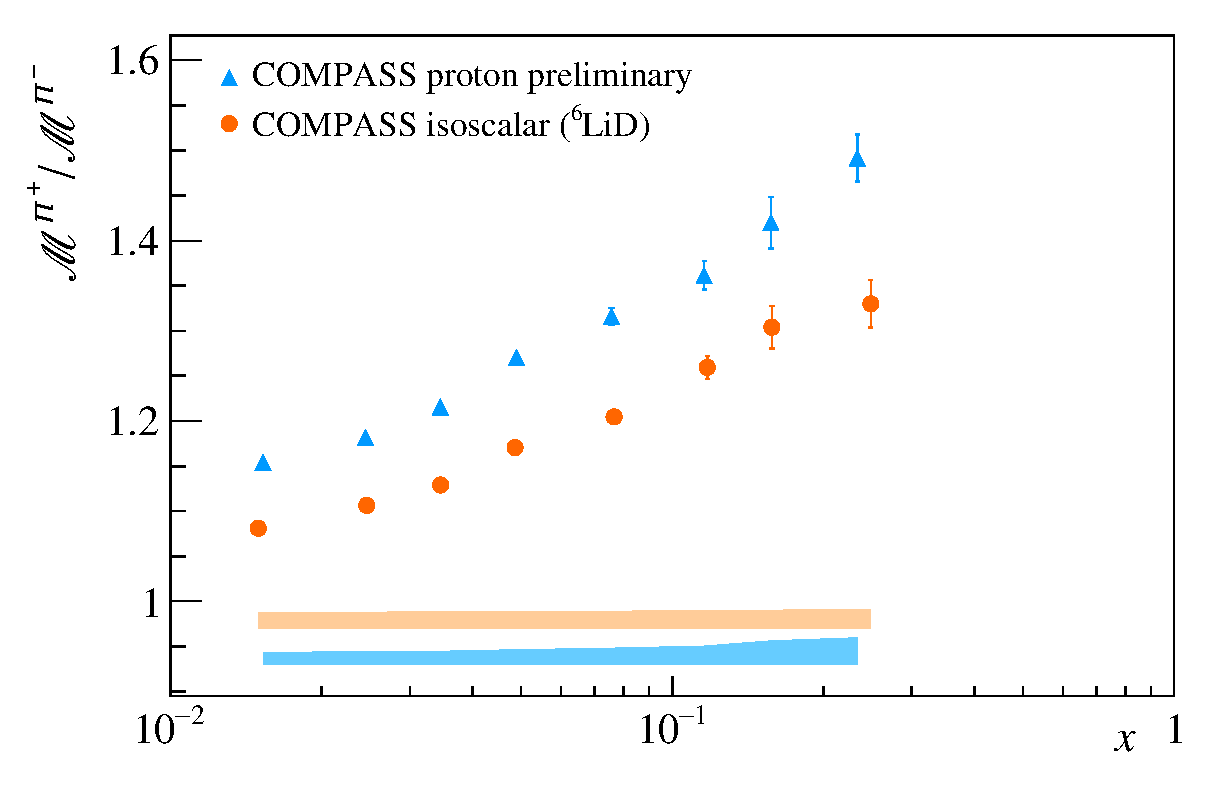
\includegraphics[scale=0.5]{./gfx/Mult_pi_ratio_noH.eps}
	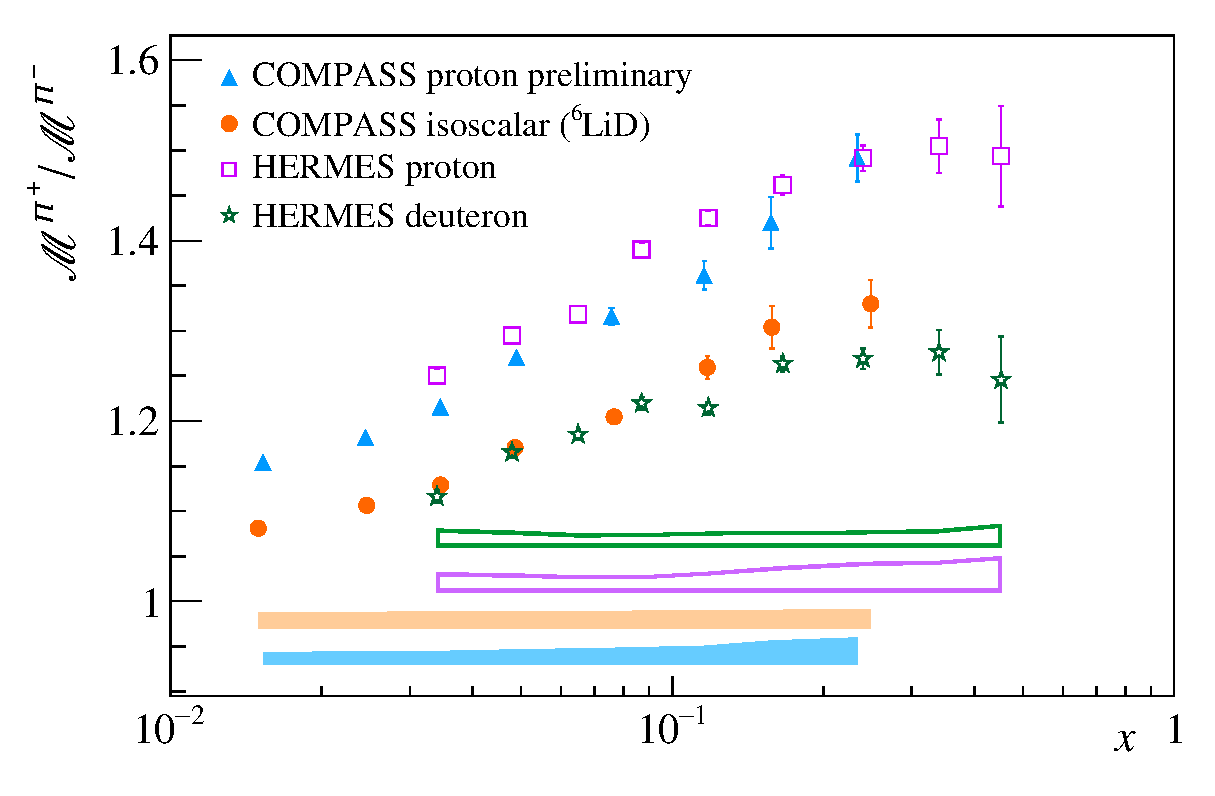
\includegraphics[scale=0.5]{./gfx/Mult_pi_ratio.eps}
	\caption{Ratio of $\frac{\mathscr{M}^{\pi^+}}{\mathscr{M}^{\pi^-}}$ from COMPASS for a proton target (blue closed points) and an isoscalar target (orange closed points) and from HERMES for a proton target (violet open points) and a deuteron target (green open points).}
	\label{pic:piratio}
\end{figure}

The COMPASS results for proton and isoscalar targets are compared to HERMES results for proton and deuteron targets. On all the $x$ range, the proton results for pions are compatible within error bars, as were the deuteron results, while for kaons discrepancies between COMPASS and HERMES results for both proton and deuteron/isoscalar targets are seen. A lead to reconcile the results is to look for hadron mass correction \cite{Accardi}, which sizeably redce the apparent large discrepancy between the measurement. In addition to this, while the pion multiplicities were found to be well described both in LO and NLO pQCD, this was not the case for kaon multiplicities. The region of large $z$ appears to be problematic for kaons. Investigations on these subjects were conducted by the COMPASS collaboration on the kaon ratio versus $z$ for large $z$ \cite{MarcinPubli} and tensions with pQCD prediction were observed. Moreover a strong $\nu$ dependence of the ratio was found and this dependence may explain the discrepancy to HERMES. HERMES data points are generally not obtained at the same $<\nu>$ than in COMPASS but when taking data points with the exact same kinematics, the results for kaon multiplicities ratio are agreeing. As for the tension with pQCD prediction, a high-$z$ ($z$ $>$ $0.75$) dependence of the ratio with a missing mass parameter $M_X = \sqrt{M^2_p + 2M_p \nu (1-z) - Q^2 (1-z)^2}$ was found. Thus, the ratio is in fact a function of $\nu$ and $z$. This points to the need of a correction within the pQCD formalism to take into account the phase-space available for the hadronisation of the target remnants. Moreover, for other experiments than COMPASS, deviations may even appear at lower $z$.

\begin{figure}[!h]
  \centering
	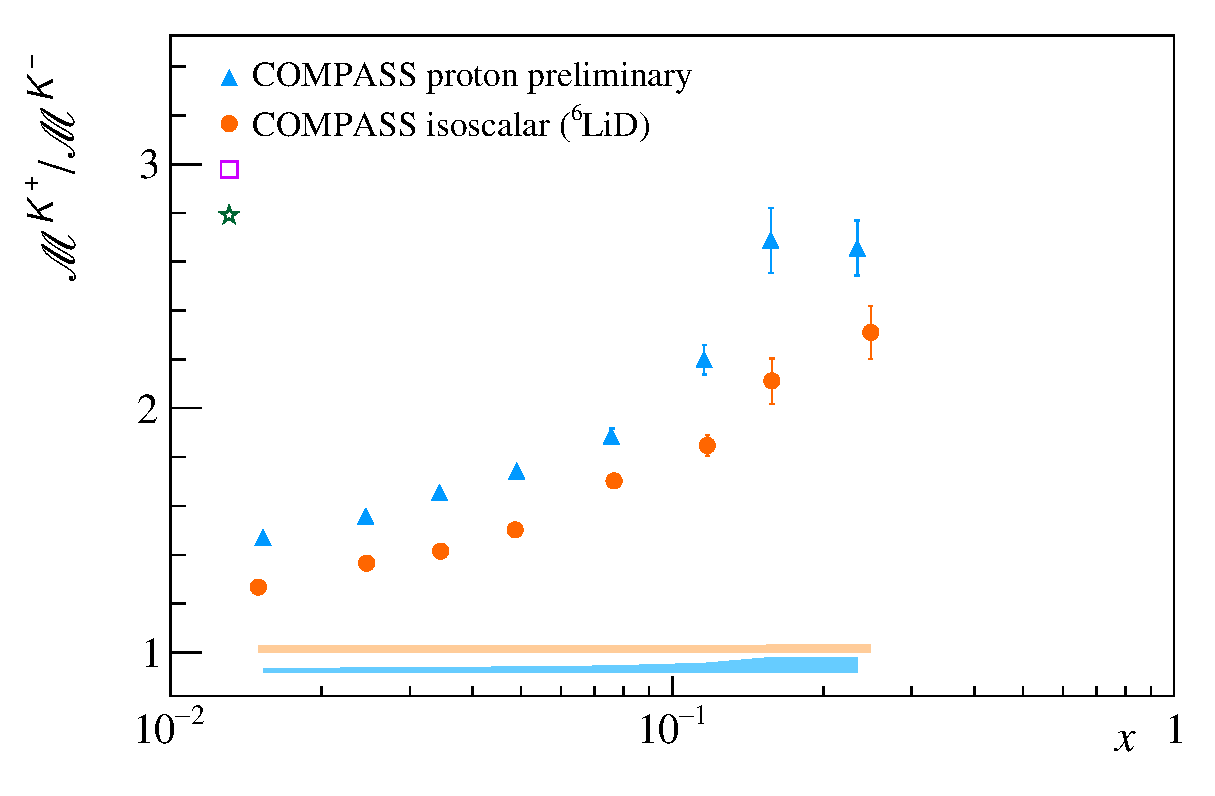
\includegraphics[scale=0.5]{./gfx/Mult_k_ratio_noH.eps}
	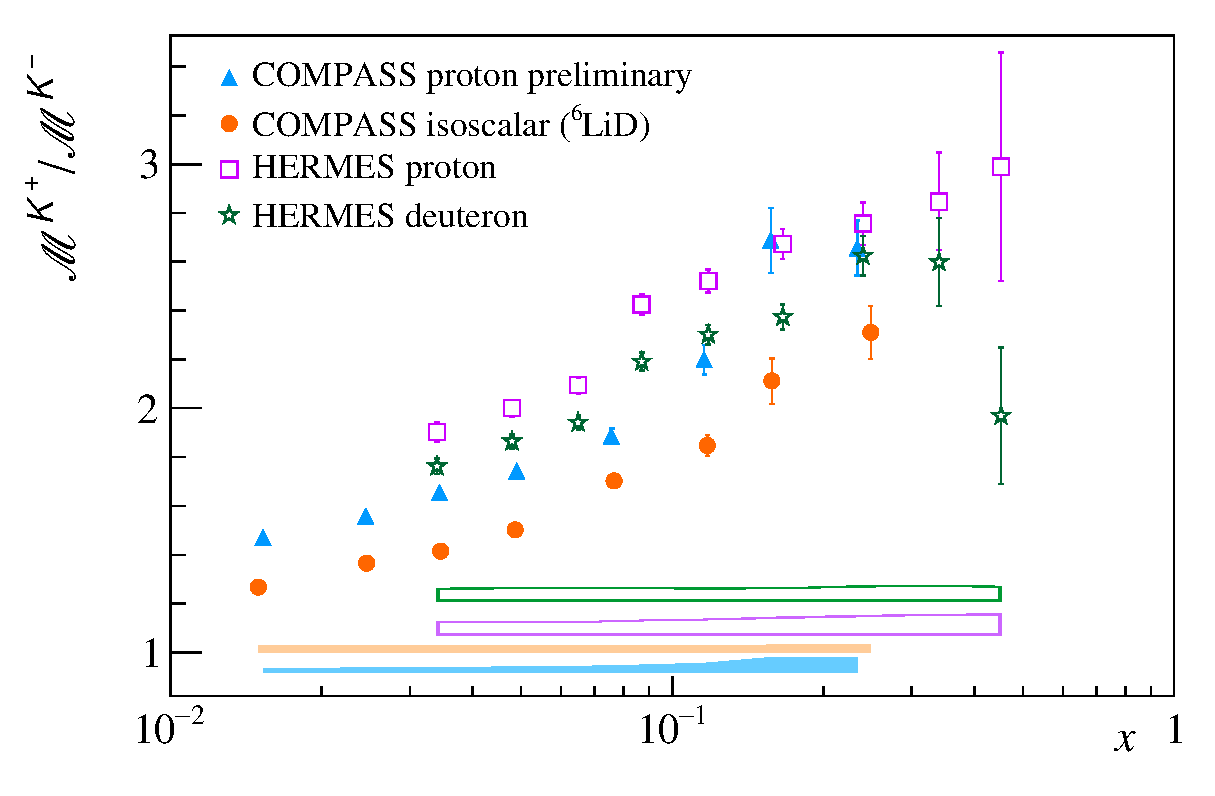
\includegraphics[scale=0.5]{./gfx/Mult_k_ratio.eps}
	\caption{Ratio of $\frac{\mathscr{M}^{K^+}}{\mathscr{M}^{K^-}}$ from COMPASS for a proton target (blue closed points) and an isoscalar target (orange closed points) and from HERMES for a proton target (violet open points) and a deuteron target (green open points).}
	\label{pic:kratio}
\end{figure}

\begin{figure}[!h]
  \centering
	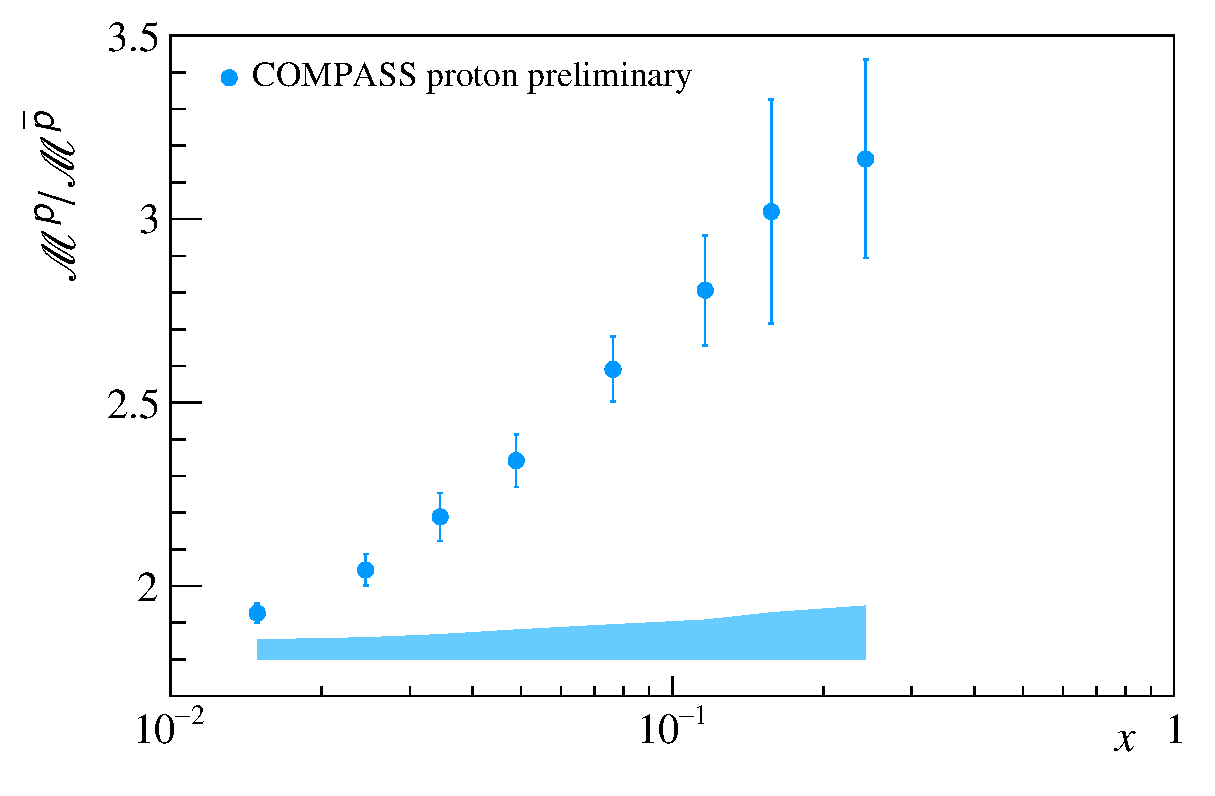
\includegraphics[scale=0.48]{./gfx/Mult_p_ratio.eps}
	\caption{Ratio of $\frac{\mathscr{M}^{p}}{\mathscr{M}^{\overline{p}}}$ from COMPASS for a proton target (blue closed points).}
	\label{pic:pratio}
\end{figure}

\subsection{Sum of charged hadron multiplicities}

In Figs.~\ref{pic:hsum} to \ref{pic:psum}, the $\mathscr{M}^{h^+}+\mathscr{M}^{h^-}$ from COMPASS is depicted for a proton target (blue triangle) and for an isoscalar target (orange circles). The same sum from HERMES is presented for a proton target (violet open squares) and a deuteron target (green open stars) for charged pions and charged kaons.

\begin{figure}[!h]
  \centering
	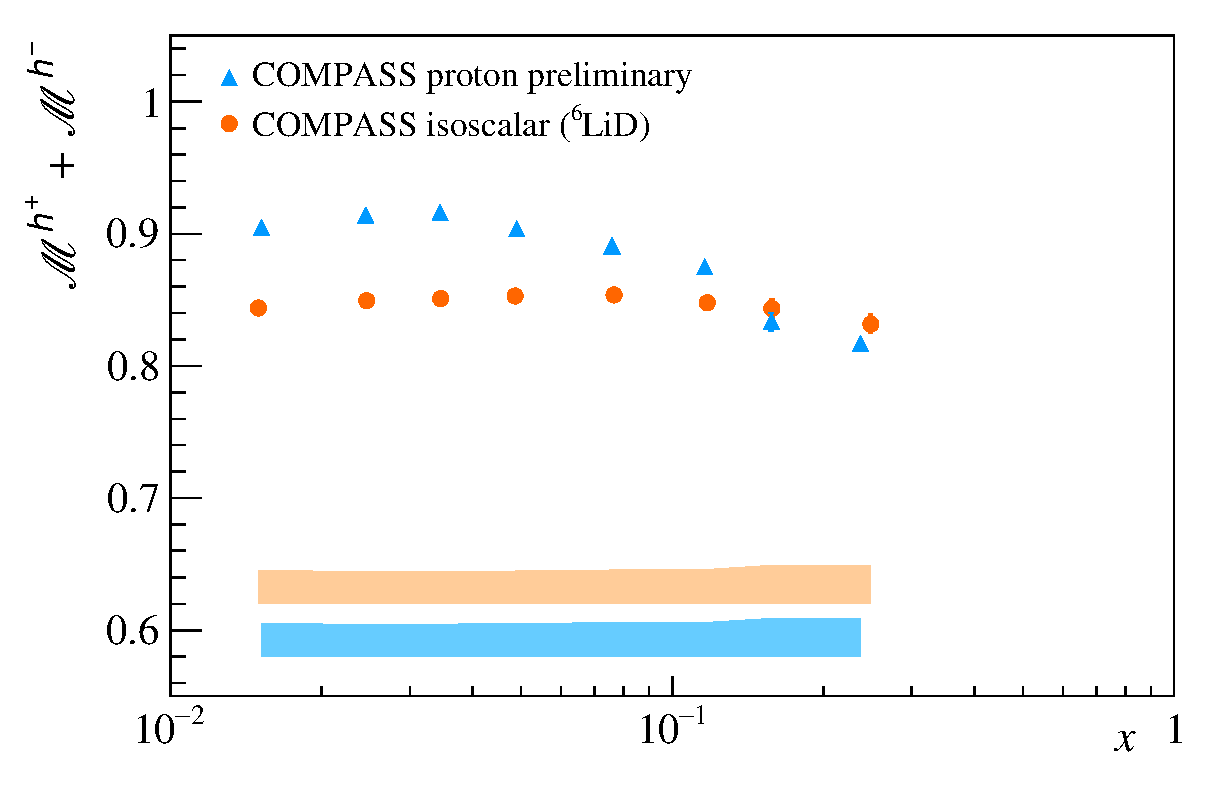
\includegraphics[scale=0.5]{./gfx/Mult_h_sum.eps}
	\caption{Sum of $\mathscr{M}^{h^+}+\mathscr{M}^{h^-}$ from COMPASS for a proton target (blue closed points) and an isoscalar target (orange closed points).}
	\label{pic:hsum}
\end{figure}

\begin{figure}[!h]
  \centering
	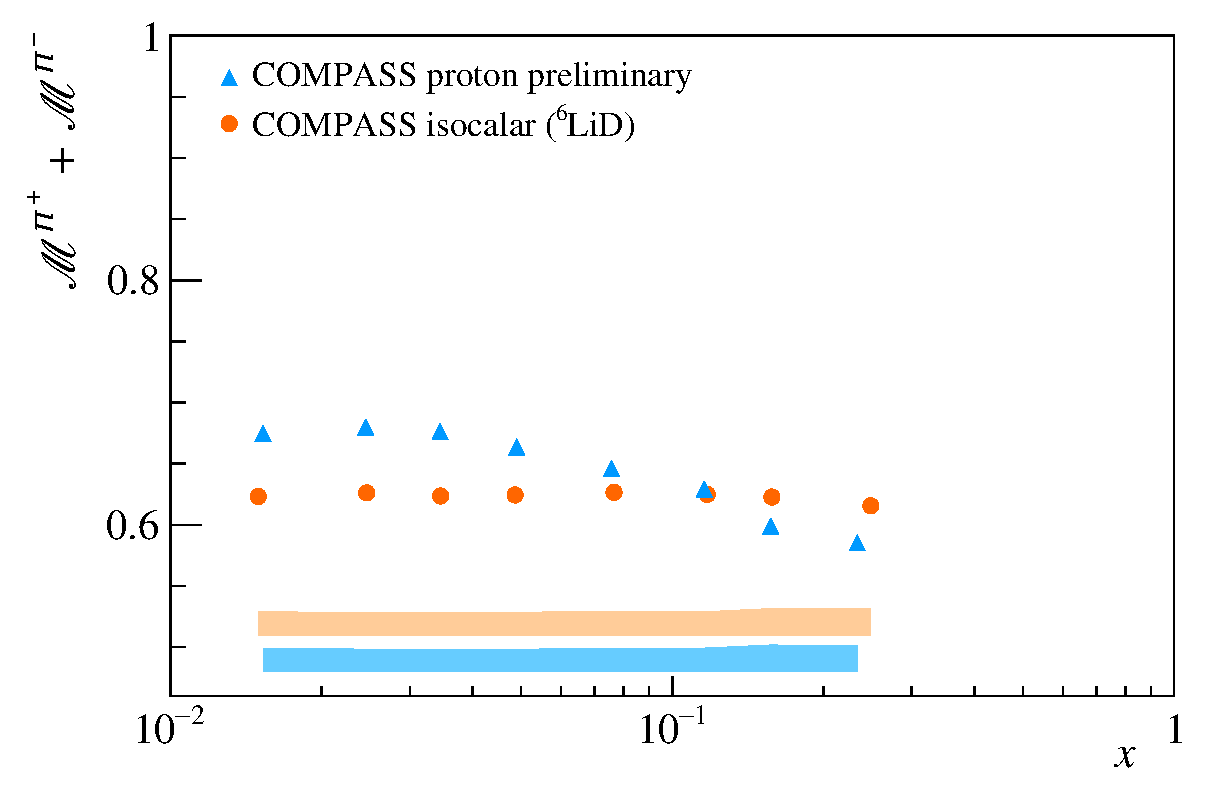
\includegraphics[scale=0.5]{./gfx/Mult_pi_sum_noH.eps}
  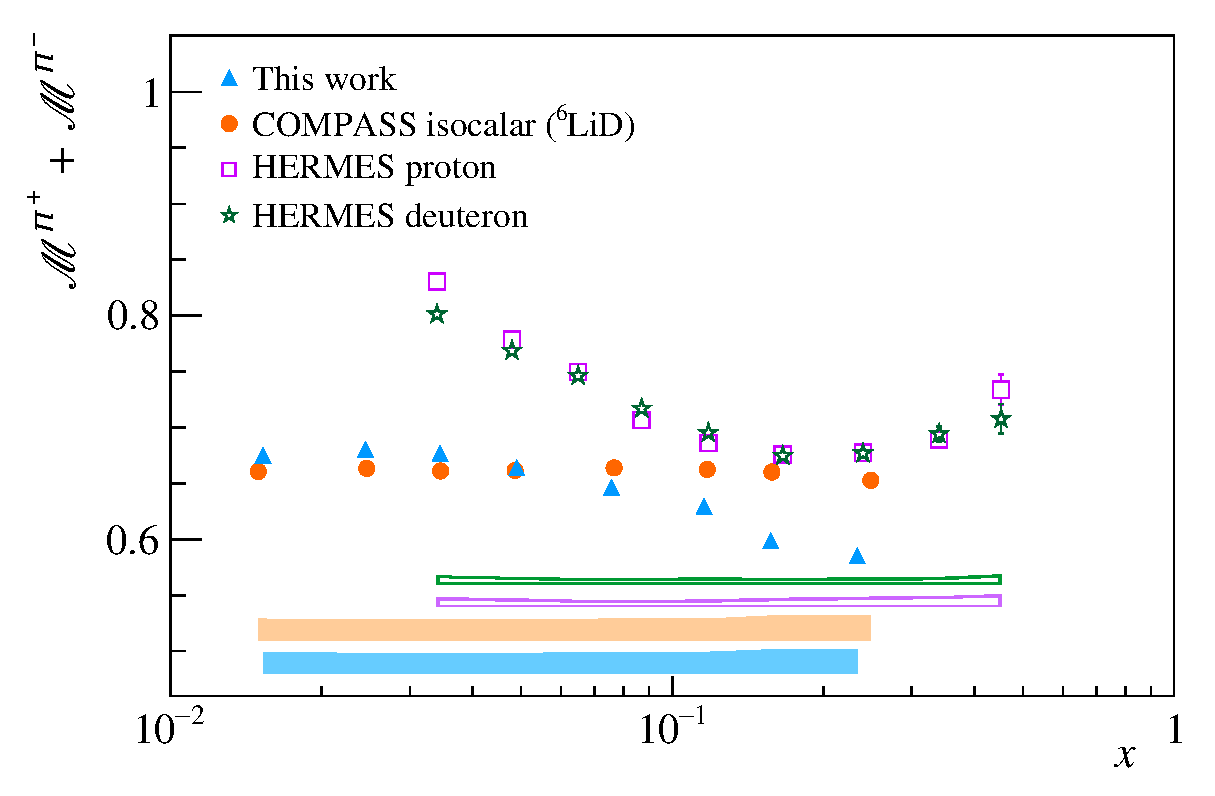
\includegraphics[scale=0.5]{./gfx/Mult_pi_sum.eps}
  \caption{Sum of $\mathscr{M}^{\pi^+}+\mathscr{M}^{\pi^-}$ from COMPASS for a proton target (blue closed points) and an isoscalar target (orange closed points) and from HERMES for a proton target (violet open points) and a deuteron target (green open points).}
  \label{pic:pisum}
\end{figure}

\begin{figure}[!h]
  \centering
	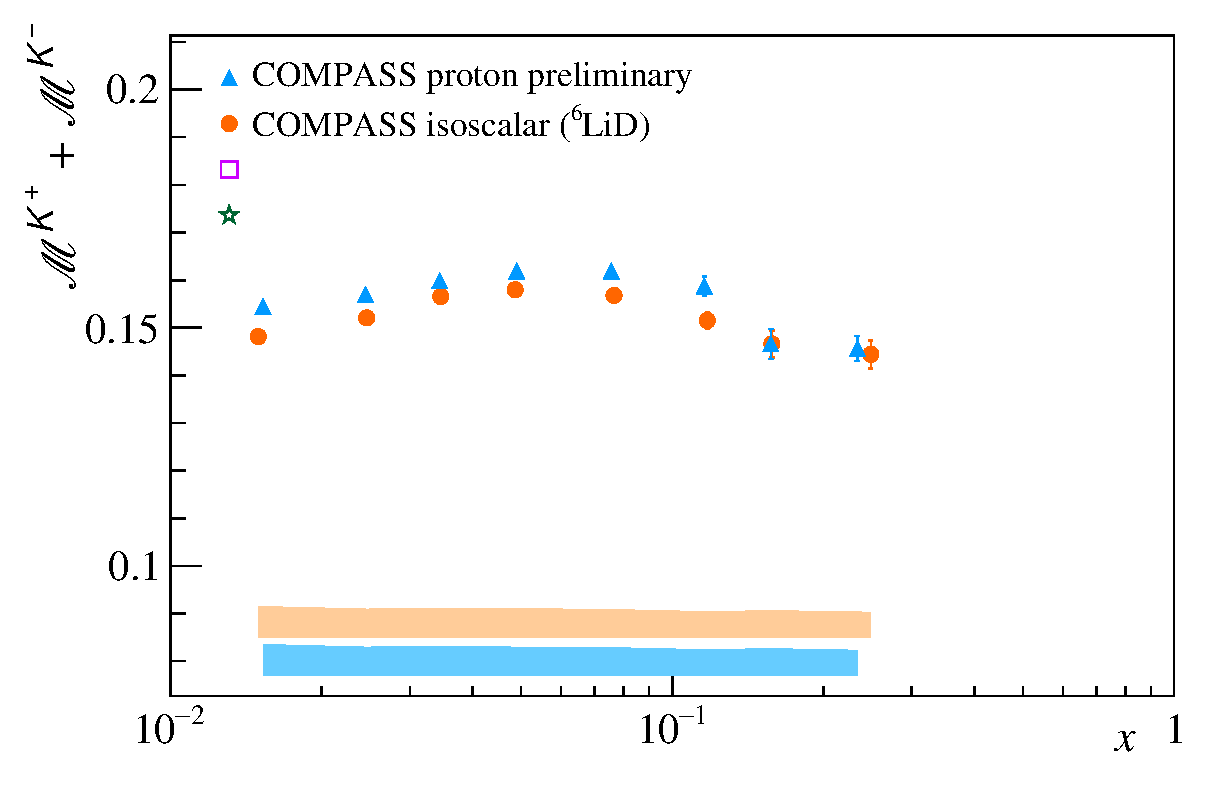
\includegraphics[scale=0.5]{./gfx/Mult_k_sum_noH.eps}
  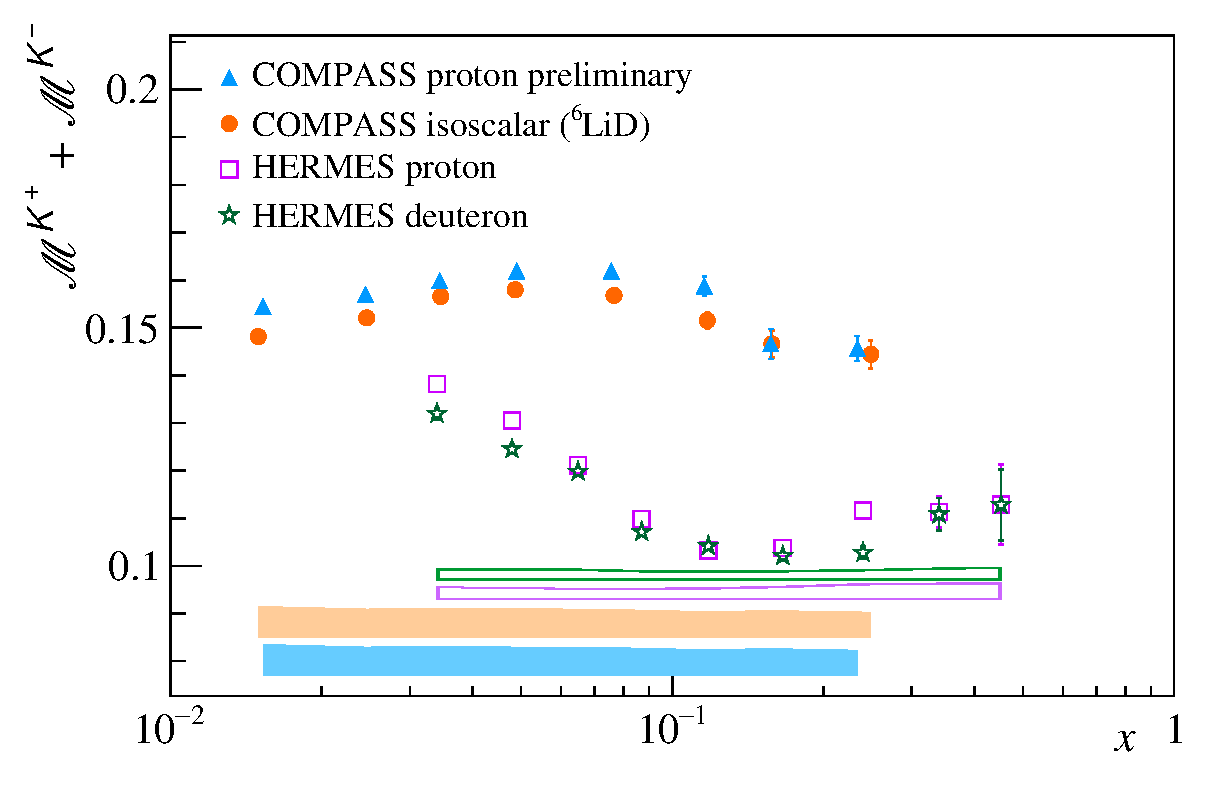
\includegraphics[scale=0.5]{./gfx/Mult_k_sum.eps}
  \caption{Sum of $\mathscr{M}^{K^+}+\mathscr{M}^{K^-}$ from COMPASS for a proton target (blue closed points) and an isoscalar target (orange closed points) and from HERMES for a proton target (violet open points) and a deuteron target (green open points).}
  \label{pic:ksum}
\end{figure}

\begin{figure}[!h]
  \centering
	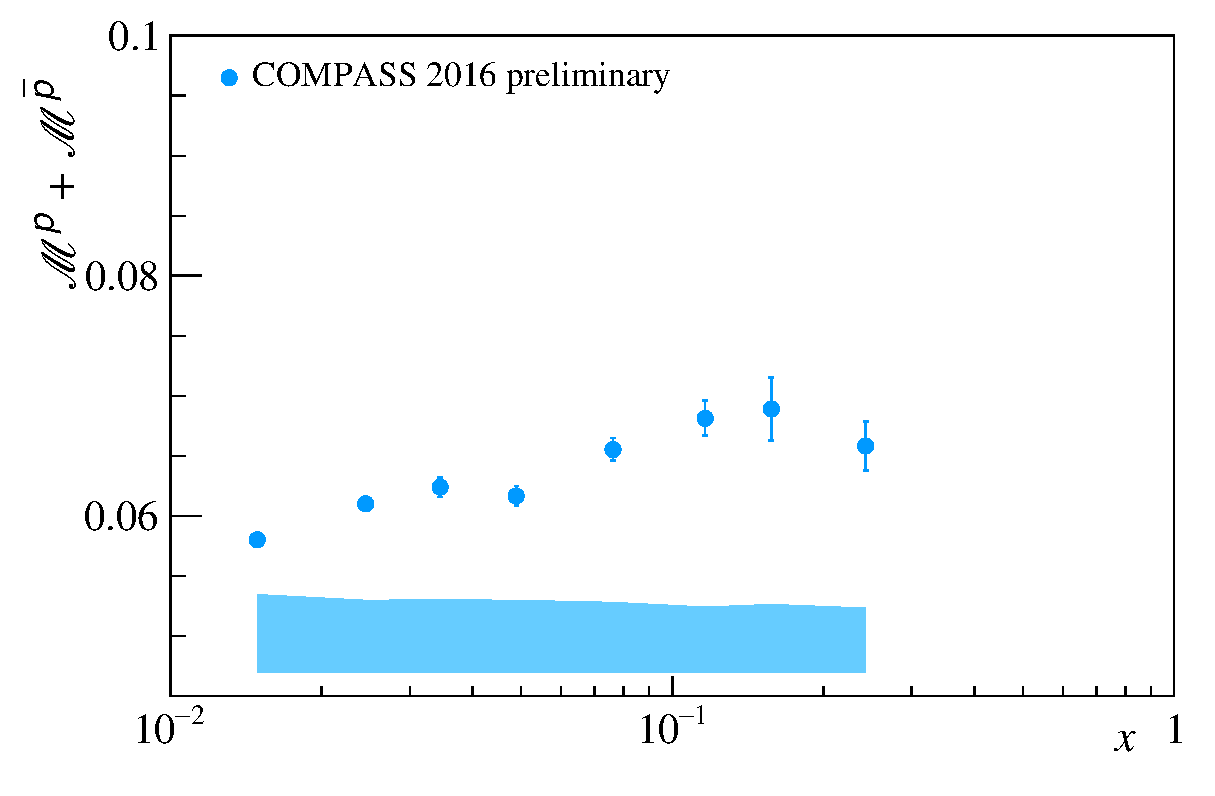
\includegraphics[scale=0.5]{./gfx/Mult_p_sum.eps}
	\caption{Sum of $\mathscr{M}^{p}+\mathscr{M}^{\overline{p}}$ for COMPASS on proton target (blue closed points).}
	\label{pic:psum}
\end{figure}

For a proton target, the charged pion multiplicities integrated over $z$ can be expressed at LO pQCD as :
%
\begin{equation}\label{eq:pisum}
  \mathscr{M}^{\pi^+}+\mathscr{M}^{\pi^-} = \mathscr{D}^{\pi}_{fav} + \mathscr{D}^{\pi}_{unf} - \frac{S}{U+D+S} \left( \mathscr{D}^{\pi}_{fav} - \mathscr{D}^{\pi}_{unf} \right),
\end{equation}
%
where $U$ = $4u+4\bar{u}$, $D$ = $d+\bar{d}$, $S$ = $us+\bar{s}$ and $\mathscr{D}^K(Q^2) = \int D^K(z,Q^2) dz $. As $\frac{S}{U+D+S}$ is small and the $Q^2$ dependence of $\mathscr{D}^{\pi}_{fav} + \mathscr{D}^{\pi}_{unf}$ is weak, the pion multiplicity sum is expected to be almost flat. The same reasoning can be done for the isoscalar case :
%
\begin{equation}
  \mathscr{M}^{\pi^+}+\mathscr{M}^{\pi^-} = \mathscr{D}^{\pi}_{fav} + \mathscr{D}^{\pi}_{unf} - \frac{2S}{5U'+2S} \left( \mathscr{D}^{\pi}_{fav} - \mathscr{D}^{\pi}_{unf} \right),
\end{equation}
%
where $U'$ = $u+\bar{u}+d+\bar{d}$. The expression of the sum for protons is the same than for pions for both targets. Thus the same conclusions can be made.

Similarly for kaons, for a proton target :
%
\begin{equation}
  \mathscr{M}^{K^+}+\mathscr{M}^{K^-} = \mathscr{D}^K_{fav}+\mathscr{D}^K_{unf}+\left[\frac{(s+\bar{s})\left( \mathscr{D}^K_{str}-\mathscr{D}^K_{fav} \right) + (d+\bar{d})\left( \mathscr{D}^K_{unf}-\mathscr{D}^K_{fav} \right)}{4(u+\bar{u}) + d + \bar{d} + s + \bar{s}} \right].
\end{equation}
%
At high value of $x$, the sea content of the nucleon can be neglected :
%
\begin{equation}
  \mathscr{M}^{K^+}+\mathscr{M}^{K^-} = \mathscr{D}^K_{fav}+\mathscr{D}^K_{unf}+\left[\frac{d\left( \mathscr{D}^K_{unf}-\mathscr{D}^K_{fav} \right)}{4u + d} \right],
\end{equation}
%
and taking as approximation $u=2d$ :
%
\begin{equation}
  \mathscr{M}^{K^+}+\mathscr{M}^{K^-} = \frac{8\mathscr{D}^K_{fav}+10\mathscr{D}^K_{unf}}{9}.
\end{equation}
%
For the isoscalar case :
%
\begin{equation}\label{eq:ksum}
  \mathscr{M}^{K^+}+\mathscr{M}^{K^-} = \frac{U\mathscr{D}^K_U+S\mathscr{D}^K_S}{5U+2S},
\end{equation}
%

The sum of charged pion (hence charged hadron as hadrons are mostly pions) multiplicity for a proton target should lie at the same level than COMPASS results for an isoscalar target, while for charged kaon the result for a proton target should be slightly ($\sim$$5-10$\%) above results on isoscalar target. These expectations are obtained by evaluating the multiplicities for both targets with Eqs.~\ref{eq:pisum} to \ref{eq:ksum} taking DSS07 \cite{DSS07} LO fragmentation functions for hadrons and integrate them over $z$ from $0.2$ to $0.85$ and taking PDFs from MSTW08 \cite{MSTW08}. At high $x$ for the hadron and pion results on proton target, the sum should be flat as for the results on isoscalar target. As seen in Chapter~\ref{ch:CF} the MC description of the data should still be improved to better simulate the $\theta_h$ dependence of the data. The discrepancy between COMPASS results and HERMES results for pions and kaons, both for a proton and deuteron targets, has to be noted. They lie well above the COMPASS points for pions and well below the COMPASS points for kaons and exhibit a different $x$ behaviour. Towards low $x$, COMPASS data show a flat behaviour, unlike the rise that is suggested by the HERMES data. Though this discrepancy cannot be explained by the mean $Q^2$ of multiplicity sets (of $\sim$ $3-5$ (GeV/$c$)$^2$ for COMPASS data and $\sim$ $1.5$ (GeV/$c$)$^2$ for HERMES) as there is no $Q^2$ evolution of the multiplicity sum. A possible explanation for kaons comes from the fact that HERMES was operating at a lower $\nu$ than in COMPASS and it was found that there might be phase space limitation effects which may be larger in the case of HERMES than in COMPASS, while it is already seen for $z>0.75$ data for COMPASS \cite{MarcinPubli}. They lie well below the COMPASS points and exhibit a different $x$ behaviour.

\newpage

\section{Summary}

The final unidentified hadron ($h^{\pm}$), pion ($\pi^{\pm}$), kaon ($K^{\pm}$) and proton/antiproton ($p/\bar{p}$) multiplicities extracted from $2016$ COMPASS data of muon deep inelastic scattering on a pure proton (lH$_2$) target were presented as a function of $z$ and in bins of $x$ and $y$. Averaging these results over $y$, two dimensional projection are obtained. The subsequent integration over $z$ allows the comparison of the sum and ratio of charged hadron multiplicities with other experiments results like HERMES \cite{HERMESMult}. Comparisons are also made with COMPASS results for an isoscalar target \cite{COMPASS2006Pi,COMPASS2006K}. For the ratio, every results are in agreement with the expectations. The discrepancy that was already observed for the kaon ratio between COMPASS and HERMES for a deuteron/isoscalar target is also present for a proton target. For the sum, the results for hadrons and pions differs from the expectations in the high $x$ region. Overall, all the results for a proton target for the sum seem to suffer from a drop at high $x$, particularly visible on hadrons and pions, which should be flat. The kaons seem to be less harmed by this issue. The cause of this drop is still under investigation. Nevertheless, comparing with HERMES results, a great discrepancy is observed in the shape for both pions and kaons. + improved results 
